\setchapterimage{figure/Chapter6封面图}
\setchapterintro{}
\chapter{定性理论初步}

\section{动力系统概念}\label{sec:动力系统概念}

在上一章研究的微分方程组中，如果右端函数只依赖于状态变量
$\vect{x}$，即
\[
	\dfrac{\dd\vect{x}}{\dd t}=\vect{f}(\vect{x}),
	\qquad \vect{x}\in\R^n,
\]
则称它为\textbf{自治微分方程组}或\textbf{自治系统}。

\begin{definition}\label{def:相空间向量场与轨道}
	状态变量 $\vect{x}$ 所在的空间 $\R^n$ 称为自治系统的
	\textbf{相空间}；相空间中每一点 $\vect{x}$ 处的向量
	$\vect{f}(\vect{x})$ 构成自治系统的\textbf{向量场}；解曲线在
	相空间中的像称为自治系统的\textbf{轨道}。
\end{definition}

\begin{definition}\label{def:平衡点与闭轨}
	若 $\vect{x}_0\in\R^n$ 满足
	\[
		\vect{f}(\vect{x}_0)=\vect{0},
	\]
	则称 $\vect{x}_0$ 为自治系统的\textbf{平衡点}，也称为
	\textbf{奇点}。此时从 $\vect{x}_0$ 出发的解是常值解
	$\vect{x}(t)\equiv\vect{x}_0$。

	若非常值解 $\vect{\varphi}(t;t_0,\vect{x}_0)$ 是 $t$ 的周期函数，
	则它在相空间中的轨道是一条闭曲线，称为\textbf{闭轨}或
	\textbf{周期轨}。
\end{definition}

自治系统的解具有以下基本性质，这些性质是非自治系统所不具备的。

\begin{proposition}\label{thm:自治系统解的基本性质}
	设自治系统满足解的存在唯一性条件，并且每个解的存在区间均为
	$(-\infty,+\infty)$。则其解
	$\vect{\varphi}(t;t_0,\vect{x}_0)$ 具有下列性质：

	\textnormal{(i)} \textbf{积分曲线的平移不变性}：对任意常数
	$\tau$，函数
	$\vect{\varphi}(t+\tau;t_0,\vect{x}_0)$ 也是该自治系统的解，且
	\[
		\vect{\varphi}(t-t_0;0,\vect{x}_0)
		\equiv\vect{\varphi}(t;t_0,\vect{x}_0).
	\]
	因此，初始时刻取为 $0$ 的解
	\[
		\vect{\varphi}(t,\vect{x}_0)
		\mathrel{:=}\vect{\varphi}(t;0,\vect{x}_0)
	\]
	的性质代表了该自治系统一切解的性质。

	\textnormal{(ii)} \textbf{群性质}：
	\[
		\vect{\varphi}(0,\vect{x}_0)=\vect{x}_0,
		\qquad
		\vect{\varphi}\bigl(t,\vect{\varphi}(s,\vect{x}_0)\bigr)
		=\vect{\varphi}(t+s,\vect{x}_0),
		\qquad \forall t,s\in\R.
	\]

	\textnormal{(iii)} \textbf{轨道唯一性}：通过相空间中的任意一点，
	只有该自治系统唯一的一条轨道。
\end{proposition}

\begin{proof}
	性质 \textnormal{(i)} 的前半部分可由自治系统直接验证。对任意
	$(t_0,\vect{x}_0)$，函数
	\[
		\vect{x}=\vect{\varphi}(t-t_0;0,\vect{x}_0)
	\]
	也是自治系统的解，并且与
	$\vect{\varphi}(t;t_0,\vect{x}_0)$ 满足同一初值条件
	$\vect{x}(t_0)=\vect{x}_0$。由解的唯一性，必有
	\[
		\vect{\varphi}(t;t_0,\vect{x}_0)
		\equiv\vect{\varphi}(t-t_0;0,\vect{x}_0).
	\]

	由性质 \textnormal{(i)}，
	$\vect{\varphi}\bigl(t,\vect{\varphi}(s,\vect{x}_0)\bigr)$ 和
	$\vect{\varphi}(t+s,\vect{x}_0)$ 都是自治系统的解。令 $t=0$，有
	\[
		\vect{\varphi}\bigl(0,\vect{\varphi}(s,\vect{x}_0)\bigr)
		=\vect{\varphi}(s,\vect{x}_0),
	\]
	故这两个解满足相同的初值条件。由解的唯一性，
	\[
		\vect{\varphi}\bigl(t,\vect{\varphi}(s,\vect{x}_0)\bigr)
		=\vect{\varphi}(t+s,\vect{x}_0),
	\]
	性质 \textnormal{(ii)} 得证。

	对于性质 \textnormal{(iii)}，设由
	$\vect{\varphi}(t-t_0,\vect{x}_0)$ 和
	$\vect{\varphi}(t-\widetilde{t}_0,\widetilde{\vect{x}}_0)$ 所确定的
	两条轨道相交，则存在 $t_1,t_2$，使得
	\[
		\vect{\varphi}(t_1-t_0,\vect{x}_0)
		=\vect{\varphi}(t_2-\widetilde{t}_0,\widetilde{\vect{x}}_0).
	\]
	由群性质，
	\begin{align*}
		\vect{\varphi}(t-t_0,\vect{x}_0)
		&=\vect{\varphi}\bigl(
		t-t_1,\vect{\varphi}(t_1-t_0,\vect{x}_0)
		\bigr)\\
		&=\vect{\varphi}\bigl(
		t-t_1,\vect{\varphi}(t_2-\widetilde{t}_0,
		\widetilde{\vect{x}}_0)
		\bigr)\\
		&=\vect{\varphi}
		(t-t_1+t_2-\widetilde{t}_0,\widetilde{\vect{x}}_0).
	\end{align*}
	这表明两解在相空间中由相同的几何点组成，即两条轨道重合。因此，
	自治系统的两条轨道要么完全重合，要么永不相交。
\end{proof}

上述定理假设自治系统的每个解都在 $(-\infty,+\infty)$ 上存在。
若原自治系统不满足这一条件，可以考虑归一化系统
\[
	\dfrac{\dd\vect{x}}{\dd t}
	=\dfrac{\vect{f}(\vect{x})}
	{\sqrt{1+\norm{\vect{f}(\vect{x})}^2}}.
\]
原自治系统与归一化系统在相空间中具有相同的轨道。另一方面，归一化
系统的右端满足
\[
	\norm{
	\dfrac{\vect{f}(\vect{x})}
	{\sqrt{1+\norm{\vect{f}(\vect{x})}^2}}
	}\leq1,
\]
所以由定理 \ref{thm:解的延拓定理}，归一化系统的解的存在区间为
$(-\infty,+\infty)$。因此，在研究自治系统的轨道结构时，不妨假设
它的解都在 $(-\infty,+\infty)$ 上存在。

下面说明两个系统具有相同轨道。设
$\vect{x}=\vect{\psi}(t)$ 是归一化系统满足初值条件
$\vect{x}(0)=\vect{x}_0$ 的解，令
\[
	s=w(t)\mathrel{:=}
	\int_0^t
	\dfrac{\dd\tau}
	{\sqrt{1+\norm{\vect{f}(\vect{\psi}(\tau))}^2}}.
\]
由于 $w'(t)>0$，故 $s=w(t)$ 有光滑的反函数 $t=w^{-1}(s)$。令
\[
	\vect{\phi}(s)=\vect{\psi}\bigl(w^{-1}(s)\bigr),
\]
则
\[
	\dfrac{\dd\vect{\phi}}{\dd s}
	=\dfrac{\vect{\psi}'(t)}{w'(t)}
	=\vect{f}(\vect{\phi}(s)),
	\qquad
	\vect{\phi}(0)=\vect{x}_0.
\]
所以，若把原自治系统的自变量记为 $s$，则
$\vect{x}=\vect{\phi}(s)$ 是它满足初值条件
$\vect{x}(0)=\vect{x}_0$ 的解。从几何上看，
$\vect{\phi}(s)$ 与 $\vect{\psi}(t)$ 在相空间中表示同一条曲线，只是
参数表示不同。这就证明了两个系统具有相同的轨道。

现在将定理 \ref{thm:自治系统解的基本性质} 中解的性质归纳起来。简记
\[
	\vect{\varphi}^{t}(\vect{x})
	\mathrel{:=}\vect{\varphi}(t,\vect{x}),
\]
则单参数变换族
$\{\vect{\varphi}^{t}:t\in\R\}$ 满足：

\textnormal{(1)} $\vect{\varphi}^{t}:\R^n\to\R^n$ 是连续的；

\textnormal{(2)} $\vect{\varphi}^{0}$ 为恒同变换，即
$\vect{\varphi}^{0}(\vect{x})\equiv\vect{x}$；

\textnormal{(3)}
$\vect{\varphi}^{t}\circ\vect{\varphi}^{s}
=\vect{\varphi}^{t+s}$。

\begin{definition}\label{def:动力系统与流}
	满足上述三条性质的单参数连续变换族
	$\{\vect{\varphi}^{t}:t\in\R\}$ 称为一个\textbf{动力系统}，
	也称为\textbf{流}。由于参数 $t$ 在 $\R$ 中连续取值，它也称为
	\textbf{连续动力系统}。若参数 $t$ 仅在 $\Z$ 中取值，则称
	$\{\vect{\varphi}^{t}:t\in\Z\}$ 为\textbf{离散动力系统}。
\end{definition}

对于非自治系统
\[
	\dfrac{\dd\vect{x}}{\dd t}=\vect{f}(t,\vect{x}),
\]
上述性质一般不再成立。然而，在高一维的相空间中仍可以定义相应的
动力系统。事实上，在 $(\vect{x},\theta)$ 所在的相空间
$\R^n\times\R$ 上考虑自治系统
\[
	\begin{cases}
		\dfrac{\dd\vect{x}}{\dd t}=\vect{f}(\theta,\vect{x}),\\[6pt]
		\dfrac{\dd\theta}{\dd t}=1.
	\end{cases}
\]
该系统与原非自治系统等价，称为原系统的\textbf{扭扩系统}
（suspension system）。

\section{Lyapunov 稳定性}\label{sec:Lyapunov稳定性}

考虑微分方程组
\[
	\dfrac{\dd\vect{x}}{\dd t}=\vect{f}(t,\vect{x}),
\]
设 $\vect{x}=\vect{\varphi}(t)$ 是它在区间 $[t_0,+\infty)$ 上有定义的
一个特解。

\begin{definition}\label{def:Lyapunov稳定性}
	称解 $\vect{x}=\vect{\varphi}(t)$ 是 \textbf{Lyapunov 稳定的}，
	如果对任意 $\varepsilon>0$，都存在
	$\delta=\delta(t_0,\varepsilon)>0$，使得只要
	\[
		\norm{\vect{x}_0-\vect{\varphi}(t_0)}<\delta,
	\]
	满足初值条件 $\vect{x}(t_0)=\vect{x}_0$ 的解
	$\vect{x}=\vect{x}(t;t_0,\vect{x}_0)$ 就在
	$[t_0,+\infty)$ 上有定义，并且
	\[
		\norm{
		\vect{x}(t;t_0,\vect{x}_0)-\vect{\varphi}(t)
		}<\varepsilon,
		\qquad \forall t\geq t_0.
	\]

	若 $\vect{\varphi}(t)$ 是 Lyapunov 稳定的，并且存在常数
	$\delta_0>0$，使得当
	$\norm{\vect{x}_0-\vect{\varphi}(t_0)}<\delta_0$ 时，
	\[
		\lim_{t\to+\infty}
		\norm{
		\vect{x}(t;t_0,\vect{x}_0)-\vect{\varphi}(t)
		}=0,
	\]
	则称它是\textbf{渐近稳定的}。此时，
	$\vect{\varphi}(t_0)$ 的 $\delta_0$ 邻域称为一个\textbf{吸引区域}；
	若可取 $\delta_0=+\infty$，则称该解是\textbf{全局渐近稳定的}。

	若存在 $\varepsilon>0$，使得对任意 $\delta>0$，都能找到满足
	$\norm{\vect{x}_0-\vect{\varphi}(t_0)}<\delta$ 的初值
	$\vect{x}_0$ 以及某个 $t_1>t_0$，使
	\[
		\norm{
		\vect{x}(t_1;t_0,\vect{x}_0)-\vect{\varphi}(t_1)
		}=\varepsilon,
	\]
	则称解 $\vect{x}=\vect{\varphi}(t)$ 是\textbf{不稳定的}。
\end{definition}

渐近稳定包含两层含义：附近的解始终保持接近，即稳定性；并且最终趋于
所考察的解，即吸引性。三种情形可用下面的简化示意图表示。

\begin{figure}[htbp]
	\centering
	\begin{tikzpicture}[x=1cm,y=1cm,>=Stealth]
		\begin{scope}[shift={(0,0)}]
			\draw (0,0) circle (1.55);
			\draw (0,0) circle (1.02);
			\draw (0,0) circle (0.42);
			\fill (0,0) circle (1.3pt);
			\draw[->,thick]
				plot[smooth,tension=0.8] coordinates
				{(0.25,0.15) (0.62,0.48) (0.42,0.78) (-0.28,0.66)
				(-0.68,0.2) (-0.42,-0.55) (0.35,-0.65)};
			\draw[->] (0.04,0.02) -- (0.92,0.02) node[midway,above] {$\varepsilon$};
			\draw[->] (0.02,-0.03) -- (-0.38,-0.15) node[midway,below] {$\delta$};
			\node at (1.22,-1.16) {$G$};
			\node[below] at (0,-1.78) {稳定};
		\end{scope}

		\begin{scope}[shift={(4.15,0)}]
			\draw (0,0) circle (1.55);
			\draw (0,0) circle (1.02);
			\draw (0,0) circle (0.42);
			\fill (0,0) circle (1.3pt);
			\draw[->,thick]
				plot[smooth,tension=0.8] coordinates
				{(-0.78,0.52) (-0.62,-0.42) (0.38,-0.68) (0.68,0.05)
				(0.18,0.46) (-0.35,0.15) (-0.1,-0.18) (0.02,-0.04)};
			\draw[->] (0.04,0.02) -- (0.92,0.02) node[midway,above] {$\varepsilon$};
			\draw[->] (0.02,-0.03) -- (-0.38,-0.15) node[midway,below] {$\delta$};
			\node at (1.22,-1.16) {$G$};
			\node[below] at (0,-1.78) {渐近稳定};
		\end{scope}

		\begin{scope}[shift={(8.3,0)}]
			\draw (0,0) circle (1.55);
			\draw (0,0) circle (1.02);
			\draw (0,0) circle (0.42);
			\fill (0,0) circle (1.3pt);
			\draw[->,thick]
				plot[smooth,tension=0.8] coordinates
				{(0.25,-0.05) (0.52,-0.35) (0.9,-0.58) (1.35,-0.38)
				(1.72,-0.05)};
			\draw[->] (0.04,0.02) -- (0.92,0.02) node[midway,above] {$\varepsilon$};
			\draw[->] (0.02,-0.03) -- (-0.38,-0.15) node[midway,below] {$\delta$};
			\node at (1.22,-1.16) {$G$};
			\node[below] at (0,-1.78) {不稳定};
		\end{scope}
	\end{tikzpicture}
	\caption{零解的稳定性、渐近稳定性与不稳定性}
	\label{fig:零解的三种稳定性情形}
\end{figure}

下面针对零解给出稳定性的判别方法。任一特解
$\vect{x}=\vect{\varphi}(t)$ 的稳定性问题，都可以通过变换
\[
	\vect{z}=\vect{x}-\vect{\varphi}(t)
\]
归结为零解的稳定性问题。事实上，原方程化为
\[
	\dfrac{\dd\vect{z}}{\dd t}
	=\widetilde{\vect{f}}(t,\vect{z})
	\mathrel{:=}
	\vect{f}\bigl(t,\vect{z}+\vect{\varphi}(t)\bigr)
	-\vect{f}\bigl(t,\vect{\varphi}(t)\bigr),
\]
且 $\widetilde{\vect{f}}(t,\vect{0})=\vect{0}$，所以原方程的特解
$\vect{\varphi}(t)$ 对应于变换后方程的零解。

判断稳定性的基本方法是研究方程的线性近似。设
$\vect{f}(t,\vect{0})=\vect{0}$，并且 $\vect{f}$ 关于
$\vect{x}$ 具有二阶连续偏导数。将 $\vect{f}(t,\vect{x})$ 关于
$\vect{x}$ 在 $\vect{0}$ 处作 Taylor 展开，可将方程写成
\[
	\dfrac{\dd\vect{x}}{\dd t}
	=A(t)\vect{x}+\vect{R}(t,\vect{x}),
\]
其中 $A(t)$ 是对 $t\geq t_0$ 连续的 $n\times n$ 阶矩阵函数，
$\vect{R}(t,\vect{x})$ 在区域
\[
	G=\left\{
	(t,\vect{x})\in\R^{n+1}:
	t\geq t_0,
	\norm{\vect{x}}\leq M
	\right\}
\]
上连续，关于 $\vect{x}$ 满足局部 Lipschitz 条件，并且对
$t\geq t_0$ 一致地满足
\[
	\vect{R}(t,\vect{0})\equiv\vect{0},
	\qquad
	\lim_{\norm{\vect{x}}\to0}
	\dfrac{\norm{\vect{R}(t,\vect{x})}}
	{\norm{\vect{x}}}=0.
\]

为了研究零解的稳定性，自然要先考察其线性部分
\[
	\dfrac{\dd\vect{x}}{\dd t}=A(t)\vect{x},
\]
它称为原方程关于零解的\textbf{线性变分方程组}或
\textbf{线性近似方程组}。

\begin{lemma}\label{lem:线性系统零解稳定性判据}
	设 $X(t)$ 是线性方程组满足 $X(t_0)=I$ 的基本解矩阵。

	\textnormal{(i)} 零解稳定，当且仅当该方程组的所有解在
	$t\geq t_0$ 时均有界，即存在常数 $K>0$，使
	\[
		\norm{X(t)}\leq K,
		\qquad \forall t\geq t_0.
	\]

	\textnormal{(ii)} 零解渐近稳定，当且仅当
	\[
		\lim_{t\to+\infty}\norm{X(t)}=0.
	\]
\end{lemma}

\begin{proof}
	先证 \textnormal{(i)} 的必要性。设零解稳定。取一个固定的
	$\varepsilon_0>0$，由稳定性可找到 $\delta_0>0$，使任一解
$\vect{x}(t)$ 只要 $\norm{\vect{x}(t_0)}<\delta_0$，便有
	\[
		\norm{\vect{x}(t)}<\varepsilon_0,
		\qquad \forall t\geq t_0.
	\]
	对任意非零初值 $\vect{x}_0$，令
	\[
		\vect{y}(t)
		\mathrel{:=}
		\dfrac{\delta_0}{2\norm{\vect{x}_0}}\vect{x}(t).
	\]
	由齐次线性方程组的线性性，$\vect{y}(t)$ 仍是解，且
	$\norm{\vect{y}(t_0)}<\delta_0$。因此
	\[
		\norm{X(t)\vect{x}_0}
		<\dfrac{2\varepsilon_0}{\delta_0}
		\norm{\vect{x}_0}.
	\]
	特别地，依次取 $\vect{x}_0$ 为 $\R^n$ 的标准正交基向量，便知
	$X(t)$ 的每一列均一致有界，从而 $X(t)$ 有界。

	反之，若 $\norm{X(t)}\leq K$，则满足初值
	$\vect{x}(t_0)=\vect{x}_0$ 的解为
	$\vect{x}(t)=X(t)\vect{x}_0$。任给 $\varepsilon>0$，取
	$\delta=\varepsilon/K$，便有
	\[
		\norm{\vect{x}(t)}
		\leq K\norm{\vect{x}_0}<\varepsilon,
		\qquad t\geq t_0,
	\]
	故零解稳定。

	再证 \textnormal{(ii)}。若 $\norm{X(t)}\to0$，则 $X(t)$ 在
	$[t_0,+\infty)$ 上有界，由 \textnormal{(i)} 知零解稳定；同时
	对任意初值 $\vect{x}_0$，
	\[
		\norm{\vect{x}(t)}
		\leq\norm{X(t)}\norm{\vect{x}_0}\longrightarrow0,
	\]
	故零解渐近稳定。反之，若零解渐近稳定，则存在一个吸引邻域。
	对每个标准基向量 $\vect{e}_j$，取充分小的常数 $c>0$，使
	$c\vect{e}_j$ 落在该吸引邻域内，于是
	$cX(t)\vect{e}_j\to\vect{0}$。因此 $X(t)$ 的每一列都趋于
	$\vect{0}$，从而 $\norm{X(t)}\to0$。
\end{proof}

当 $A(t)$ 为常矩阵 $A$ 时，由引理
\ref{lem:线性系统零解稳定性判据} 和第四章常系数齐次线性方程组的
解结构，可以得到下列结论。

\begin{theorem}\label{thm:常系数线性系统零解稳定性判据}
	设 $A$ 为常矩阵，则：

	\textnormal{(i)} 线性方程组
	\[
		\dfrac{\dd\vect{x}}{\dd t}=A\vect{x}
	\]
	的零解渐近稳定，当且仅当 $A$ 的全部特征根的实部均为负数。

	\textnormal{(ii)} 零解稳定，当且仅当 $A$ 的全部特征根的实部均
	非正，并且实部为零的特征根所对应的 Jordan 块都是一阶的。

	\textnormal{(iii)} 零解不稳定，当且仅当 $A$ 至少有一个特征根的
	实部为正，或者至少有一个实部为零的特征根所对应的 Jordan 块的
	阶数大于 $1$。
\end{theorem}

\begin{proof}
	由定理 \ref{thm:常系数线性方程组的矩阵指数解}，满足
	$X(t_0)=I$ 的基本解矩阵为
	\[
		X(t)=\mathrm{e}^{(t-t_0)A}.
	\]
	把 $A$ 化为 Jordan 标准形。若
	$J=\lambda I+N$ 是一个 $m$ 阶 Jordan 块，其中
	$N^m=0$，则
	\[
		\mathrm{e}^{(t-t_0)J}
		=\mathrm{e}^{\lambda(t-t_0)}
		\left[
		I+(t-t_0)N+\cdots+
		\dfrac{(t-t_0)^{m-1}}{(m-1)!}N^{m-1}
		\right].
	\]
	因此，每个 Jordan 块的增长或衰减由指数因子
	$\mathrm{e}^{\operatorname{Re}\lambda(t-t_0)}$ 与至多
	$m-1$ 次的多项式因子共同决定。

	若所有特征根的实部均为负，则指数衰减快于任意多项式增长，故
	$\norm{X(t)}\to0$；反之，只要存在实部非负的特征根，便有相应的
	解不趋于零。由引理 \ref{lem:线性系统零解稳定性判据} 的
	\textnormal{(ii)}，结论 \textnormal{(i)} 成立。

	若所有特征根的实部均非正，且实部为零的特征根所对应的 Jordan
	块均为一阶，则负实部对应的块趋于零，零实部对应的块保持有界，
	所以 $X(t)$ 有界，零解稳定。反之，实部为正的特征根产生指数增长；
	实部为零而阶数大于 $1$ 的 Jordan 块产生非零的多项式增长项。
	这两种情形都会使 $X(t)$ 无界。再由引理
	\ref{lem:线性系统零解稳定性判据} 的 \textnormal{(i)}，即得
	结论 \textnormal{(ii)} 和 \textnormal{(iii)}。
\end{proof}

下面回到非线性方程
\[
	\dfrac{\dd\vect{x}}{\dd t}
	=A\vect{x}+\vect{R}(t,\vect{x}),
\]
其中 $A$ 为常矩阵，且余项满足前述小量条件。

\begin{theorem}\label{thm:线性近似决定非线性系统稳定性}
	设 $A$ 为常矩阵，并且
	\[
		\lim_{\norm{\vect{x}}\to0}
		\dfrac{\norm{\vect{R}(t,\vect{x})}}
		{\norm{\vect{x}}}=0
	\]
	对 $t\geq t_0$ 一致成立，则：

	\textnormal{(i)} 当 $A$ 的全部特征根的实部均为负时，非线性方程
	的零解渐近稳定；

	\textnormal{(ii)} 当 $A$ 至少有一个特征根的实部为正时，非线性
	方程的零解不稳定。
\end{theorem}

\begin{proof}
	只证明结论 \textnormal{(i)}。取
	$\norm{\vect{x}_0}<M$，则满足初值条件
	$\vect{x}(t_0)=\vect{x}_0$ 的解
	$\vect{x}(t)=\vect{\varphi}(t)$ 对充分靠近 $t_0$ 的 $t$ 存在。
	设其最大存在区间为 $[t_0,t_1)$。由常数变易公式，
	\[
		\vect{\varphi}(t)
		=\mathrm{e}^{(t-t_0)A}\vect{x}_0
		+\int_{t_0}^t
		\mathrm{e}^{(t-s)A}
		\vect{R}(s,\vect{\varphi}(s))\dd s.
	\]

	由于 $A$ 的全部特征根的实部均为负，存在常数 $K>0$、
	$\rho>0$，使得
	\[
		\norm{\mathrm{e}^{(t-t_0)A}}
		\leq K\mathrm{e}^{-\rho(t-t_0)},
		\qquad t\geq t_0.
	\]
	这个估计可由第四章的 Jordan 标准形直接得到：对每个 Jordan 块，
	指数衰减因子可以控制相应的多项式因子。

	对上述 $K,\rho$，任取
	\[
		0<\alpha<\dfrac{\rho}{2K}.
	\]
	由余项的小量条件，可以取充分小的 $M>0$，使当
	$\norm{\vect{x}}<M$ 时，
	\[
		\norm{\vect{R}(t,\vect{x})}
		\leq\alpha\norm{\vect{x}}.
	\]
	由连续性，不妨仍用 $[t_0,t_1)$ 表示满足
	$\norm{\vect{\varphi}(t)}<M$ 的极大区间。于是对
	$t\in[t_0,t_1)$，
	\[
		\norm{\vect{\varphi}(t)}
		\leq K\norm{\vect{x}_0}\mathrm{e}^{-\rho(t-t_0)}
		+K\alpha\int_{t_0}^t
		\mathrm{e}^{-\rho(t-s)}
		\norm{\vect{\varphi}(s)}\dd s.
	\]
	等价地，
	\[
		\mathrm{e}^{\rho(t-t_0)}\norm{\vect{\varphi}(t)}
		\leq K\norm{\vect{x}_0}
		+K\alpha\int_{t_0}^t
		\mathrm{e}^{\rho(s-t_0)}
		\norm{\vect{\varphi}(s)}\dd s.
	\]
	由 Gronwall 不等式，
	\[
		\mathrm{e}^{\rho(t-t_0)}\norm{\vect{\varphi}(t)}
		\leq K\norm{\vect{x}_0}
		\mathrm{e}^{K\alpha(t-t_0)},
		\qquad t\in[t_0,t_1).
	\]
	因此
	\[
		\norm{\vect{\varphi}(t)}
		\leq K\norm{\vect{x}_0}
		\mathrm{e}^{-(\rho-K\alpha)(t-t_0)}
		<K\norm{\vect{x}_0}
		\mathrm{e}^{-\dfrac{\rho}{2}(t-t_0)}.
	\]
	取正数 $\sigma<M/K$，并考虑满足
	$\norm{\vect{x}_0}<\sigma$ 的初值。上式表明
	$\norm{\vect{\varphi}(t)}<K\sigma<M$，所以由解的延拓定理必有
	$t_1=+\infty$，并且
	\[
		\lim_{t\to+\infty}\vect{\varphi}(t)=\vect{0}.
	\]
	同时，任给 $\varepsilon>0$，再取
	$\norm{\vect{x}_0}<\min\{\sigma,\varepsilon/K\}$，便有
	$\norm{\vect{\varphi}(t)}<\varepsilon$ 对所有 $t\geq t_0$ 成立。
	故零解渐近稳定。
\end{proof}

由定理 \ref{thm:线性近似决定非线性系统稳定性} 可知，为了判定零解
是否渐近稳定，需要判断矩阵 $A$ 的全部特征根的实部是否均为负数。
当矩阵阶数较大时，无需求出全部特征根的精确值，可以使用下面的
Routh--Hurwitz 判据。

\begin{theorem}(Routh--Hurwitz 定理)\label{thm:RouthHurwitz定理}
	实系数多项式
	\[
		\lambda^n+a_1\lambda^{n-1}+\cdots
		+a_{n-1}\lambda+a_n
	\]
	的全部根的实部均为负数，当且仅当下面的 Routh--Hurwitz 矩阵
	\[
		D_n\mathrel{:=}
		\begin{pmatrix}
			a_1&1&0&0&\cdots&0\\
			a_3&a_2&a_1&1&\ddots&\vdots\\
			a_5&a_4&a_3&a_2&\ddots&0\\
			\vdots&\vdots&\vdots&\vdots&\ddots&1\\
			a_{2n-1}&a_{2n-2}&a_{2n-3}&a_{2n-4}&\cdots&a_n
		\end{pmatrix}_{n\times n}
	\]
	的全部顺序主子式均为正，即
	\[
		\Delta_1\mathrel{:=}a_1>0,
		\qquad
		\Delta_2\mathrel{:=}
		\begin{vmatrix}
			a_1&1\\
			a_3&a_2
		\end{vmatrix}>0,
	\]
	\[
		\Delta_3\mathrel{:=}
		\begin{vmatrix}
			a_1&1&0\\
			a_3&a_2&a_1\\
			a_5&a_4&a_3
		\end{vmatrix}>0,
		\qquad \ldots,
		\qquad
		\Delta_n\mathrel{:=}\det D_n>0.
	\]
	这里约定 $a_0=1$，并且当 $k<0$ 或 $k>n$ 时 $a_k=0$。
\end{theorem}

Routh--Hurwitz 定理的证明在我矩阵论的笔记里。

\section{Lyapunov 直接法}\label{sec:Lyapunov直接法}

上一节的线性近似法不能完全处理矩阵 $A$ 具有实部为零的特征根时的
临界情形，因为此时方程的高阶项也可能影响稳定性。Lyapunov 直接法
不需求出微分方程的解，而是通过构造适当的辅助函数直接判断稳定性，
因而也称为 Lyapunov 第二方法。

为简单起见，只考虑自治系统
\[
	\dfrac{\dd\vect{x}}{\dd t}=\vect{f}(\vect{x}),
\]
其中 $\vect{x}\in\R^n$，$\vect{f}(\vect{0})=\vect{0}$，并且
$\vect{f}$ 在区域
\[
	G=\left\{
	\vect{x}\in\R^n:\norm{\vect{x}}\leq M
	\right\}
\]
内连续可微。于是相应初值问题的解存在且唯一，并且
$\vect{x}=\vect{0}$ 是该系统的零解。

\begin{definition}\label{def:正定与半正定函数}
	设连续实函数 $V(\vect{x})$ 定义在闭区域
	\[
		\left\{
		\vect{x}\in\R^n:\norm{\vect{x}}\leq M_1
		\right\},
		\qquad 0<M_1\leq M,
	\]
	且 $V(\vect{0})=0$。

	若恒有 $V(\vect{x})\geq0$，则称 $V$ 为\textbf{常正函数}或
	\textbf{半正定函数}；若对一切 $\vect{x}\neq\vect{0}$ 都有
	$V(\vect{x})>0$，则称 $V$ 为\textbf{定正函数}或
	\textbf{正定函数}。若 $-V$ 为常正函数或定正函数，则分别称
	$V$ 为\textbf{常负函数}或\textbf{定负函数}。
\end{definition}

例如，$V(x,y)=(x+y)^2$ 是常正函数，而
$V(x,y)=x^2+y^2$ 是定正函数。对于二次型
\[
	V(x,y)=ax^2+bxy+cy^2,
\]
当 $a>0$ 且 $b^2-4ac<0$ 时，它是定正函数；当 $a<0$ 且
$b^2-4ac<0$ 时，它是定负函数。

取连续可微函数 $V(\vect{x})$，沿自治系统的任一解
$\vect{x}(t)$ 求导，得到
\[
	\left.\dfrac{\dd V}{\dd t}\right|_{\vect{x}'=\vect{f}(\vect{x})}
	\mathrel{:=}
	\dfrac{\dd V(\vect{x}(t))}{\dd t}
	=\sum_{i=1}^n
	\dfrac{\partial V}{\partial x_i}
	\dfrac{\dd x_i}{\dd t}
	=\sum_{i=1}^n
	\dfrac{\partial V}{\partial x_i}f_i(\vect{x}).
\]
以下简记这个沿轨道的导数为 $\dot V(\vect{x})$。

\begin{theorem}(Lyapunov 稳定性判据)\label{thm:Lyapunov稳定性判据}
	对于上述自治系统，有以下结论：

	\textnormal{(i)} 若存在定正函数 $V(\vect{x})$，使
	$\dot V(\vect{x})$ 为常负函数，则零解稳定。

	\textnormal{(ii)} 若存在定正函数 $V(\vect{x})$，使
	$\dot V(\vect{x})$ 为定负函数，则零解渐近稳定。

	\textnormal{(iii)} 若存在定正函数 $V(\vect{x})$，使
	$\dot V(\vect{x})$ 为定正函数，则零解不稳定。

	\textnormal{(iv)} 若存在满足 $V(\vect{0})=0$ 的连续可微函数
	$V(\vect{x})$ 和非负常数 $\mu$，使得在
	$\vect{x}=\vect{0}$ 的任意小邻域内都存在
	$\overline{\vect{x}}$，满足 $V(\overline{\vect{x}})>0$，并且
	\[
		\dot V(\vect{x}(t))
		=\mu V(\vect{x}(t))+W(\vect{x}(t)),
	\]
	其中当 $\mu=0$ 时，$W(\vect{x})$ 为定正函数；当
	$\mu\neq0$ 时，$W(\vect{x})$ 为常正函数，则零解不稳定。
\end{theorem}

满足上述稳定性判据的辅助函数 $V$ 通常称为
\textbf{Lyapunov 函数}。

\begin{proof}
	先证结论 \textnormal{(i)}。任取 $0<\varepsilon\leq M_1$。
	由 $V$ 的连续性和正定性，
	\[
		\eta(\varepsilon)
		\mathrel{:=}
		\min_{\varepsilon\leq\norm{\vect{x}}\leq M_1}
		V(\vect{x})>0.
	\]
	再由 $V(\vect{0})=0$ 及连续性，存在
	$0<\delta=\delta(\varepsilon)<\varepsilon$，使得
	\[
		\norm{\vect{x}}<\delta
		\quad\Longrightarrow\quad
		V(\vect{x})<\eta(\varepsilon).
	\]
	取 $\norm{\vect{x}_0}<\delta$，设满足初值条件
	$\vect{x}(t_0)=\vect{x}_0$ 的解为 $\vect{x}(t)$，其最大存在区间为
	$[t_0,t_1)$。由于 $\dot V\leq0$，对任意
	$t\in[t_0,t_1)$ 都有
	\[
		V(\vect{x}(t))
		\leq V(\vect{x}_0)<\eta(\varepsilon).
	\]
	由 $\eta(\varepsilon)$ 的定义及解的连续性可知，
	$\norm{\vect{x}(t)}<\varepsilon$ 在 $[t_0,t_1)$ 上成立。
	解始终留在该有界区域内，故由解的延拓定理必有
	$t_1=+\infty$。因此零解稳定。

	再证结论 \textnormal{(ii)}。由于 $\dot V$ 定负，由结论
	\textnormal{(i)}，零解已经稳定。取上面稳定性证明中的一个
	$\delta_0>0$。当 $\norm{\vect{x}_0}<\delta_0$ 时，相应解
	$\vect{x}(t)$ 对所有 $t\geq t_0$ 均有定义，并且
	$\norm{\vect{x}(t)}\leq M_1$。只需证明
	\[
		\lim_{t\to+\infty}\vect{x}(t)=\vect{0}.
	\]
	先证明
	\[
		\lim_{t\to+\infty}V(\vect{x}(t))=0.
	\]
	事实上，由于 $V(\vect{x}(t))\geq0$ 且
	$\dot V(\vect{x}(t))<0$，极限
	\[
		c\mathrel{:=}
		\lim_{t\to+\infty}V(\vect{x}(t))
	\]
	存在且 $c\geq0$。若 $c>0$，由 $V$ 的连续性、正定性以及
	$V(\vect{x}(t))\geq c$，存在 $\alpha>0$，使
	\[
		\norm{\vect{x}(t)}\geq\alpha,
		\qquad t\geq t_0.
	\]
	于是由 $\dot V$ 的连续性和定负性，
	\[
		m\mathrel{:=}
		\max_{\alpha\leq\norm{\vect{x}}\leq M_1}
		\dot V(\vect{x})<0.
	\]
	故 $\dot V(\vect{x}(t))\leq m$。在 $[t_0,t]$ 上积分，得到
	\[
		V(\vect{x}(t))
		\leq V(\vect{x}_0)+m(t-t_0).
	\]
	令 $t\to+\infty$，右端趋于 $-\infty$，与左端非负矛盾。因此
	$c=0$。

	若 $V(\vect{x}(t))\to0$ 而 $\vect{x}(t)$ 不趋于
	$\vect{0}$，由于 $\vect{x}(t)$ 有界，可取序列
	$t_k\to+\infty$，使
	$\vect{x}(t_k)\to\widetilde{\vect{x}}\neq\vect{0}$。由连续性，
	\[
		V(\widetilde{\vect{x}})
		=\lim_{k\to\infty}V(\vect{x}(t_k))=0,
	\]
	这与 $V$ 正定矛盾。故零解渐近稳定。

	最后证明结论 \textnormal{(iv)}。它同时包含结论
	\textnormal{(iii)}。任给 $0<\delta<M_1$，可取
	$\norm{\vect{x}_0}<\delta$ 且 $V(\vect{x}_0)>0$。设
	$\vect{x}(t)$ 是满足 $\vect{x}(t_0)=\vect{x}_0$ 的解。只需证明
	存在某个 $t>t_0$，使 $\norm{\vect{x}(t)}>M_1$。

	反设对所有 $t\geq t_0$ 都有
	\[
		\norm{\vect{x}(t)}\leq M_1.
	\]
	由于 $V$ 在闭球上连续，$V(\vect{x}(t))$ 必有界。另一方面，由
	常数变易公式，
	\[
		V(\vect{x}(t))
		=\mathrm{e}^{\mu(t-t_0)}
		\left[
		V(\vect{x}_0)
		+\int_{t_0}^t
		W(\vect{x}(\tau))
		\mathrm{e}^{-\mu(\tau-t_0)}\dd\tau
		\right].
	\]
	当 $\mu\neq0$ 时，$\mu>0$ 且 $W$ 常正，故
	\[
		V(\vect{x}(t))
		\geq V(\vect{x}_0)\mathrm{e}^{\mu(t-t_0)}
		\longrightarrow+\infty,
	\]
	与有界性矛盾。

	当 $\mu=0$ 时，$W$ 定正，且
	$V(\vect{x}(t))\geq V(\vect{x}_0)>0$。由 $V$ 的连续性及
	$V(\vect{0})=0$，存在 $\alpha>0$，使
	$\norm{\vect{x}(t)}\geq\alpha$。于是
	\[
		m\mathrel{:=}
		\min_{\alpha\leq\norm{\vect{x}}\leq M_1}
		W(\vect{x})>0,
	\]
	从而
	\[
		V(\vect{x}(t))
		\geq V(\vect{x}_0)+m(t-t_0)
		\longrightarrow+\infty,
	\]
	仍与有界性矛盾。因此零解不稳定。
\end{proof}

上述判据具有直观的几何意义。在二维情形中，若 $V$ 正定，则当
$c>0$ 充分小时，等值线
\[
	V(x_1,x_2)=c
\]
构成一族互不相交、相互嵌套并包围原点的闭曲线。当
$\dot V\leq0$ 时，轨道不能由闭曲线族的内部穿到外部；当
$\dot V<0$ 时，轨道由外向内穿过等值线并渐近趋于原点；在不稳定的
情形中，轨道则由内向外离开这些等值线。

\begin{figure}[htbp]
	\centering
	\begin{tikzpicture}[x=1cm,y=1cm,>=Stealth]
		\begin{scope}[shift={(0,0)}]
			\draw (0,0) ellipse (2.1 and 1.45);
			\draw (0,0) ellipse (1.55 and 1.05);
			\draw (0,0) ellipse (0.95 and 0.62);
			\fill (0,0) circle (1.3pt) node[above left] {$O$};
			\node[rotate=25] at (1.25,-0.72) {$V=c_3$};
			\node[rotate=25] at (0.92,-0.48) {$V=c_2$};
			\node[rotate=25] at (0.55,-0.24) {$V=c_1$};
			\node[below] at (0,-1.78) {$c_1<c_2<c_3$};
		\end{scope}

		\begin{scope}[shift={(5.5,0)}]
			\draw (0,0) ellipse (2.1 and 1.45);
			\draw (0,0) ellipse (1.55 and 1.05);
			\draw (0,0) ellipse (0.95 and 0.62);
			\fill (0,0) circle (1.3pt) node[above left] {$O$};
			\draw[->,thick]
				plot[smooth,tension=0.85] coordinates
				{(1.75,0.7) (1.1,0.9) (0.5,0.55) (0.75,0.05)
				(0.25,-0.35) (-0.2,-0.15) (-0.05,0.02)};
			\node at (1.35,-0.75) {$V=c$};
			\draw[->] (0.05,0.02) -- (0.85,0.02)
				node[midway,above] {$\delta$};
			\draw[->] (0.08,0.05) -- (-1.48,0.2)
				node[midway,above] {$\varepsilon$};
			\node[below] at (0,-1.78) {$\dot V<0$ 时轨道向内运动};
		\end{scope}
	\end{tikzpicture}
	\caption{Lyapunov 函数等值线与轨道的运动方向}
	\label{fig:Lyapunov函数等值线与轨道}
\end{figure}

在 $\dot V\leq0$ 但不定负时，还可以使用下面的判据。

\begin{theorem}\label{thm:Lyapunov半负定导数渐近稳定判据}
	若存在定正函数 $V(\vect{x})$，其沿自治系统的导数
	$\dot V(\vect{x})$ 为常负函数，并且集合
	\[
		E=\left\{
		\vect{x}:\dot V(\vect{x})=0
		\right\}
	\]
	中除零解外，不包含该自治系统的任何一条整条正半轨道，则零解
	渐近稳定。
\end{theorem}

\begin{proof}
	由定理 \ref{thm:Lyapunov稳定性判据} 的结论
	\textnormal{(i)}，零解稳定。取充分小的初值，使相应解
	$\vect{x}(t)$ 对所有 $t\geq t_0$ 都位于定义域内的一个紧球中。
	因为 $\dot V\leq0$，函数 $V(\vect{x}(t))$ 单调不增且有下界，
	所以存在极限
	\[
		\lim_{t\to+\infty}V(\vect{x}(t))=c\geq0.
	\]

	只需证明 $\vect{x}(t)\to\vect{0}$。反设不成立，则存在
	$\varepsilon>0$ 和序列 $t_k\to+\infty$，使
	$\norm{\vect{x}(t_k)}\geq\varepsilon$。由轨道有界，可取子列，仍记为
	$t_k$，使
	\[
		\vect{x}(t_k)\longrightarrow\vect{x}^{*},
		\qquad \norm{\vect{x}^{*}}\geq\varepsilon.
	\]
	记从 $\vect{x}^{*}$ 出发的解为 $\vect{y}(s)$，$s\geq0$。
	由稳定性和解的延拓定理，$\vect{y}(s)$ 在整个正半轴上有定义。
	由解对初值的连续依赖性，对每个固定的 $s\geq0$，有
	\[
		\vect{x}(t_k+s)\longrightarrow\vect{y}(s).
	\]
	另一方面，$t_k+s\to+\infty$，故由 $V$ 的连续性，
	\[
		V(\vect{y}(s))
		=\lim_{k\to\infty}V(\vect{x}(t_k+s))
		=c,
		\qquad \forall s\geq0.
	\]
	所以 $V$ 沿正半轨道 $\vect{y}(s)$ 恒为常数，从而
	$\dot V(\vect{y}(s))=0$。这说明整条正半轨道
	$\{\vect{y}(s):s\geq0\}$ 都包含在 $E$ 中。

	根据定理的假设，这条正半轨道只能是零解，因而
	$\vect{x}^{*}=\vect{0}$，这与
	$\norm{\vect{x}^{*}}\geq\varepsilon$ 矛盾。因此
	$\vect{x}(t)\to\vect{0}$。结合零解的稳定性，零解渐近稳定。
\end{proof}

\section{平面平衡点分析}\label{sec:平面平衡点分析}

前面关于平衡点 $O$ 附近轨道的“走法”，包括 $O$ 点稳定性在内的
性质，就是本节要讨论的平衡点的定性性质。考虑平面自治系统
\[
	\dfrac{\dd x}{\dd t}=X(x,y),
	\qquad
	\dfrac{\dd y}{\dd t}=Y(x,y),
\]
其中 $X(x,y)$ 和 $Y(x,y)$ 为连续函数，并对 $x,y$ 具有二阶连续偏导数，
因而系统满足解的存在唯一性条件。

若 $X(x,y)$ 与 $Y(x,y)$ 不同时为零，则可以消去自变量 $t$。当
$X(x,y)\neq0$ 时有
\[
	\dfrac{\dd y}{\dd x}=\dfrac{Y(x,y)}{X(x,y)};
\]
当 $Y(x,y)\neq0$ 时有
\[
	\dfrac{\dd x}{\dd y}=\dfrac{X(x,y)}{Y(x,y)}.
\]
这两个一阶微分方程所确定的积分曲线就是原系统的轨道。由解的
存在唯一性与对初值的连续依赖性可知，相平面上的每个非平衡点都有且
只有一条轨道通过，而且在该点的某个邻域内，轨道是一族互不相交的曲线。
称这样的点为\textbf{常点}。

因此，相图的局部结构问题集中在系统的平衡点附近。平衡点由方程组
\[
	X(x,y)=0,
	\qquad
	Y(x,y)=0
\]
确定。一个系统可以有多个平衡点，我们可分别将它们平移到原点，故下文
设所讨论的平衡点为 $O=(0,0)$。在原点作 Taylor 展开，系统可写成
\[
	\left\{
	\begin{aligned}
		\dfrac{\dd x}{\dd t}&=ax+by+R_1(x,y),\\
		\dfrac{\dd y}{\dd t}&=cx+dy+R_2(x,y),
	\end{aligned}
	\right.
\]
其中
\[
	R_j(x,y)=o\!\left(\sqrt{x^2+y^2}\right),
	\qquad j=1,2.
\]
对应的线性部分为
\[
	\left\{
	\begin{aligned}
		\dfrac{\dd x}{\dd t}&=ax+by,\\
		\dfrac{\dd y}{\dd t}&=cx+dy.
	\end{aligned}
	\right.
\]
下面先分析该线性系统平衡点的定性性质。

记其系数矩阵为
\[
	A=\begin{pmatrix}a&b\\c&d\end{pmatrix}.
\]
先考虑 $A$ 非退化的情形，即 $\det A\neq0$。此时 $A$ 在复数域中有
两个非零特征根 $\lambda_1,\lambda_2$。由 Jordan 标准形理论，存在
非奇异线性变换
\[
	\begin{pmatrix}u\\v\end{pmatrix}
	=P\begin{pmatrix}x\\y\end{pmatrix},
\]
使系统化为
\[
	\dfrac{\dd}{\dd t}\begin{pmatrix}u\\v\end{pmatrix}
	=PAP^{-1}\begin{pmatrix}u\\v\end{pmatrix}.
\]
其中 $J=PAP^{-1}$ 是下列三种实标准形之一：
\[
	\begin{pmatrix}\lambda&0\\0&\mu\end{pmatrix},
	\qquad
	\begin{pmatrix}\lambda&0\\1&\lambda\end{pmatrix},
	\qquad
	\begin{pmatrix}\alpha&\beta\\-\beta&\alpha\end{pmatrix}.
\]
这里 $\lambda,\mu,\alpha,\beta$ 均为实数，且
$\lambda\mu\beta\neq0$。前两种形式对应于 $A$ 只有实特征根的情形，
第三种形式对应于 $A$ 有一对共轭复根
$\lambda_{1,2}=\alpha\pm\mathrm{i}\beta$ 的情形。

具体的线性变换可以如下选取。若特征根
$\lambda_1=\lambda$、$\lambda_2=\mu$ 为相异实根，当 $b\neq0$ 时取
\[
	u=(d-\lambda_1)x-by,
	\qquad
	v=(d-\lambda_2)x-by;
\]
当 $c\neq0$ 时也可取
\[
	u=-cx+(a-\lambda_1)y,
	\qquad
	v=-cx+(a-\lambda_2)y.
\]
若 $\lambda_1=\lambda_2=\lambda$ 为相同实根，当 $b\neq0$ 时取
\[
	u=(\lambda-d)x+by,
	\qquad v=x;
\]
当 $c\neq0$ 时取
\[
	u=cx+(\lambda-a)y,
	\qquad v=y.
\]
若 $\lambda_{1,2}=\alpha\pm\mathrm{i}\beta$，$\beta\neq0$，则可取
\[
	u=-cx+(a-\alpha)y,
	\qquad v=\beta y,
\]
或
\[
	u=(d-\alpha)x-by,
	\qquad v=\beta x.
\]
这些变换均可将原系统化为相应标准形，而且这种线性变换不是唯一的。
由于可逆线性变换不改变平衡点的位置和相图结构，下面只讨论由三种
标准矩阵所定义的系统。

\subsection*{一、第一种标准形}

对第一种标准形分三种情形：
\[
	\begin{array}{ll}
	\textnormal{(I.1)}&\lambda=\mu,\\
	\textnormal{(I.2)}&\lambda\neq\mu\ \text{且}\ \lambda\mu>0,\\
	\textnormal{(I.3)}&\lambda\mu<0.
	\end{array}
\]

在情形 \textnormal{(I.1)} 中，系统为
\[
	\dfrac{\dd u}{\dd t}=\lambda u,
	\qquad
	\dfrac{\dd v}{\dd t}=\lambda v,
\]
其解为
\[
	u(t)=u_0e^{\lambda t},
	\qquad
	v(t)=v_0e^{\lambda t}.
\]
当 $\lambda<0$ 时轨道趋向平衡点 $O$，零解渐近稳定；当
$\lambda>0$ 时轨道远离平衡点 $O$，零解不稳定。又由
\[
	\dfrac{u}{v}=\dfrac{u_0}{v_0}
\]
可知，平衡点附近的轨道都是通过 $O$ 点的直线。这样的平衡点称为
\textbf{星形结点}（或\textbf{临界结点}）。

\begin{figure}[htbp]
	\centering
	\begin{tikzpicture}[>=Stealth,scale=.9]
		\begin{scope}[shift={(-3,0)}]
			\draw[->] (-2.1,0)--(2.1,0) node[right] {$u$};
			\draw[->] (0,-1.7)--(0,1.7) node[above] {$v$};
			\foreach \a in {0,30,...,330}{\draw[->] (\a:1.85)--(\a:.16);}
			\fill[white] (0,0) circle (2pt); \draw (0,0) circle (2pt) node[below left] {$O$};
			\node[below=7pt] at (0,-1.7) {稳定的星形结点（$\lambda<0$）};
		\end{scope}
		\begin{scope}[shift={(3,0)}]
			\draw[->] (-2.1,0)--(2.1,0) node[right] {$u$};
			\draw[->] (0,-1.7)--(0,1.7) node[above] {$v$};
			\foreach \a in {0,30,...,330}{\draw[->] (\a:.16)--(\a:1.85);}
			\fill[white] (0,0) circle (2pt); \draw (0,0) circle (2pt) node[below left] {$O$};
			\node[below=7pt] at (0,-1.7) {不稳定的星形结点（$\lambda>0$）};
		\end{scope}
	\end{tikzpicture}
	\caption{星形结点的相图}
	\label{fig:星形结点相图}
\end{figure}

在情形 \textnormal{(I.2)} 中，系统为
\[
	\dfrac{\dd u}{\dd t}=\lambda u,
	\qquad
	\dfrac{\dd v}{\dd t}=\mu v,
\]
其通解为
\[
	u(t)=u_0e^{\lambda t},
	\qquad
	v(t)=v_0e^{\mu t}.
\]
当 $\lambda<0$、$\mu<0$ 时原点渐近稳定；当 $\lambda>0$、$\mu>0$
时原点不稳定。由轨道方程
\[
	\dfrac{\dd v}{\dd u}=\dfrac{\mu}{\lambda}\dfrac{v}{u}
\]
解得
\[
	v=C|u|^{\mu/\lambda},
\]
其中 $C$ 为任意常数。因此，除坐标轴外，轨道构成一族以原点为顶点
的幂函数曲线。当 $|\lambda|<|\mu|$ 时，该曲线族与 $u$ 轴相切于
$O$；当 $|\mu|<|\lambda|$ 时，该曲线族与 $v$ 轴相切于 $O$。
坐标轴的正、负半轴也分别是系统的轨道。这样的平衡点称为
\textbf{两向结点}（或\textbf{正常结点}）。

\begin{figure}[htbp]
	\centering
	\begin{tikzpicture}[>=Stealth,scale=.86]
		\begin{scope}[shift={(-3.1,0)}]
			\draw[->] (-2.2,0)--(2.2,0) node[right] {$u$};
			\draw[->] (0,-1.75)--(0,1.75) node[above] {$v$};
			\foreach \s in {-1,1}{
				\draw[->] plot[smooth] coordinates {(2,1.35*\s) (1.25,.7*\s) (.55,.16*\s) (.12,.01*\s)};
				\draw[->] plot[smooth] coordinates {(-2,1.35*\s) (-1.25,.7*\s) (-.55,.16*\s) (-.12,.01*\s)};
			}
			\draw[->] (2,0)--(.12,0); \draw[->] (-2,0)--(-.12,0);
			\draw[->] (0,1.55)--(0,.12); \draw[->] (0,-1.55)--(0,-.12);
			\draw[fill=white] (0,0) circle (2pt) node[below left] {$O$};
			\node[below=7pt] at (0,-1.75) {稳定的两向结点（$\mu<\lambda<0$）};
		\end{scope}
		\begin{scope}[shift={(3.1,0)}]
			\draw[->] (-2.2,0)--(2.2,0) node[right] {$u$};
			\draw[->] (0,-1.75)--(0,1.75) node[above] {$v$};
			\foreach \s in {-1,1}{
				\draw[<-] plot[smooth] coordinates {(2,1.35*\s) (1.25,.7*\s) (.55,.16*\s) (.12,.01*\s)};
				\draw[<-] plot[smooth] coordinates {(-2,1.35*\s) (-1.25,.7*\s) (-.55,.16*\s) (-.12,.01*\s)};
			}
			\draw[<-] (2,0)--(.12,0); \draw[<-] (-2,0)--(-.12,0);
			\draw[<-] (0,1.55)--(0,.12); \draw[<-] (0,-1.55)--(0,-.12);
			\draw[fill=white] (0,0) circle (2pt) node[below left] {$O$};
			\node[below=7pt] at (0,-1.75) {不稳定的两向结点（$\lambda>\mu>0$）};
		\end{scope}
	\end{tikzpicture}
	\caption{两向结点的相图}
	\label{fig:两向结点相图}
\end{figure}

在情形 \textnormal{(I.3)} 中，由通解或轨道方程可知原点总是不稳定的，
并且除坐标轴外，轨道形成一族以两个坐标轴为渐近线的双曲线。当
$\lambda<0$、$\mu>0$ 时，轨道在 $t\to+\infty$ 时渐近于 $v$ 轴；
当 $\lambda>0$、$\mu<0$ 时，轨道在 $t\to+\infty$ 时渐近于 $u$ 轴。
这样的平衡点称为\textbf{鞍点}。

\begin{figure}[htbp]
	\centering
	\begin{tikzpicture}[>=Stealth,scale=.86]
		\foreach \shift/\lab in {-3.1/{\lambda<0,\ \mu>0},3.1/{\lambda>0,\ \mu<0}}{
			\begin{scope}[shift={(\shift,0)}]
				\draw[->] (-2.1,0)--(2.1,0) node[right] {$u$};
				\draw[->] (0,-1.75)--(0,1.75) node[above] {$v$};
				\foreach \sx in {-1,1}{\foreach \sy in {-1,1}{
					\draw plot[domain=.42:2,samples=35] ({\sx*\x},{\sy*.55/\x});
				}}
				\ifdim \shift pt<0pt
					\draw[->] (1.5,.37)--(.8,.69); \draw[->] (-1.5,.37)--(-.8,.69);
					\draw[->] (1.5,-.37)--(.8,-.69); \draw[->] (-1.5,-.37)--(-.8,-.69);
					\draw[->] (1.8,0)--(.2,0); \draw[->] (-1.8,0)--(-.2,0);
					\draw[->] (0,.2)--(0,1.5); \draw[->] (0,-.2)--(0,-1.5);
				\else
					\draw[<-] (1.5,.37)--(.8,.69); \draw[<-] (-1.5,.37)--(-.8,.69);
					\draw[<-] (1.5,-.37)--(.8,-.69); \draw[<-] (-1.5,-.37)--(-.8,-.69);
					\draw[<-] (1.8,0)--(.2,0); \draw[<-] (-1.8,0)--(-.2,0);
					\draw[<-] (0,.2)--(0,1.5); \draw[<-] (0,-.2)--(0,-1.5);
				\fi
				\draw[fill=white] (0,0) circle (2pt) node[below left] {$O$};
				\node[below=7pt] at (0,-1.75) {鞍点（$\lab$）};
			\end{scope}
		}
	\end{tikzpicture}
	\caption{鞍点的相图}
	\label{fig:鞍点相图}
\end{figure}

\subsection*{二、第二种标准形}

第二种标准形的矩阵具有一个二重实根，并且 Jordan 块为二阶。系统为
\[
	\dfrac{\dd u}{\dd t}=\lambda u,
	\qquad
	\dfrac{\dd v}{\dd t}=u+\lambda v.
\]
由通解容易看出，平衡点 $O$ 在 $\lambda<0$ 时渐近稳定，在
$\lambda>0$ 时不稳定。当 $u\neq0$ 时，轨道满足
\[
	\dfrac{\dd v}{\dd u}=\dfrac{1}{\lambda}+\dfrac{v}{u}.
\]
用常数变易公式得到
\[
	v=Cu+\dfrac{u}{\lambda}\ln|u|,
\]
其中 $C$ 为任意常数。因此 $\lim\limits_{u\to0}v=0$，并且 $v$ 轴的正、负
半轴本身也是轨道。又有
\[
	\lim_{u\to0}\dfrac{\dd v}{\dd u}
	=
	\begin{cases}
		+\infty,&\lambda<0,\\
		-\infty,&\lambda>0.
	\end{cases}
\]
故平衡点附近的轨道与 $v$ 轴相切于 $O$。这样的平衡点称为
\textbf{单向结点}（或\textbf{退化结点}）。

\begin{figure}[htbp]
	\centering
	\begin{tikzpicture}[>=Stealth,scale=.86]
		\begin{scope}[shift={(-3.1,0)}]
			\draw[->] (-2.2,0)--(2.2,0) node[right] {$u$};
			\draw[->] (0,-1.8)--(0,1.8) node[above] {$v$};
			\foreach \s in {-1,1}{
				\draw[->] (2,1.45*\s)..controls (1.4,.15*\s) and (1.35,-1.35*\s)..(0.06,0);
				\draw[->] (-2,-1.45*\s)..controls (-1.4,-.15*\s) and (-1.35,1.35*\s)..(-.06,0);
			}
			\draw[->] (0,1.6)--(0,.12); \draw[->] (0,-1.6)--(0,-.12);
			\draw[fill=white] (0,0) circle (2pt) node[below left] {$O$};
			\node[below=7pt] at (0,-1.8) {稳定的单向结点（$\lambda<0$）};
		\end{scope}
		\begin{scope}[shift={(3.1,0)}]
			\draw[->] (-2.2,0)--(2.2,0) node[right] {$u$};
			\draw[->] (0,-1.8)--(0,1.8) node[above] {$v$};
			\foreach \s in {-1,1}{
				\draw[<-] (2,1.45*\s)..controls (1.4,.15*\s) and (1.35,-1.35*\s)..(.06,0);
				\draw[<-] (-2,-1.45*\s)..controls (-1.4,-.15*\s) and (-1.35,1.35*\s)..(-.06,0);
			}
			\draw[<-] (0,1.6)--(0,.12); \draw[<-] (0,-1.6)--(0,-.12);
			\draw[fill=white] (0,0) circle (2pt) node[below left] {$O$};
			\node[below=7pt] at (0,-1.8) {不稳定的单向结点（$\lambda>0$）};
		\end{scope}
	\end{tikzpicture}
	\caption{单向结点的相图}
	\label{fig:单向结点相图}
\end{figure}

\subsection*{三、第三种标准形}

第三种标准形的矩阵有一对共轭复根
$\lambda_{1,2}=\alpha\pm\mathrm{i}\beta$，其中 $\beta\neq0$。取极坐标
\[
	u=r\cos\theta,
	\qquad
	v=r\sin\theta.
\]
由
\[
	\left\{
	\begin{aligned}
		\dot u&=\dot r\cos\theta-r\sin\theta\,\dot\theta,\\
		\dot v&=\dot r\sin\theta+r\cos\theta\,\dot\theta
	\end{aligned}
	\right.
\]
可得
\[
	\dot r=\dot u\cos\theta+\dot v\sin\theta,
	\qquad
	\dot\theta=\dfrac{-\dot u\sin\theta+\dot v\cos\theta}
	{\sqrt{u^2+v^2}}.
\]
于是系统化为
\[
	\dfrac{\dd r}{\dd t}=\alpha r,
	\qquad
	\dfrac{\dd\theta}{\dd t}=-\beta,
\]
从而
\[
	r(t)=\rho_0e^{\alpha t},
	\qquad
	\theta(t)=-\beta t+\delta,
\]
其中 $\rho_0,\delta$ 为任意常数。因此平衡点附近的轨道满足
\[
	r(\theta)=\left(\rho_0e^{\alpha\delta/\beta}\right)
	e^{-\alpha\theta/\beta}.
\]

当 $\alpha\neq0$ 时，轨道是一族螺线。若 $\alpha<0$，平衡点渐近
稳定；若 $\alpha>0$，平衡点不稳定。当 $\beta>0$ 时螺线顺时针旋转，
当 $\beta<0$ 时螺线逆时针旋转。这样的平衡点称为\textbf{焦点}。
当 $\alpha=0$ 时，$r(t)=\rho_0$，轨道是一族同心圆。此时平衡点稳定
但不渐近稳定，称为\textbf{中心}。

\begin{figure}[htbp]
	\centering
	\begin{tikzpicture}[>=Stealth,scale=.76]
		\begin{scope}[shift={(-4.5,0)}]
			\draw[->] (-2,0)--(2,0) node[right] {$u$}; \draw[->] (0,-1.7)--(0,1.7) node[above] {$v$};
			\draw[->,domain=0:690,samples=150,smooth,variable=\t]
				plot ({(1.9-.0025*\t)*cos(\t)},{(1.9-.0025*\t)*sin(\t)});
			\draw[fill=white] (0,0) circle (2pt) node[below left] {$O$};
			\node[below=7pt] at (0,-1.7) {稳定的焦点$\alpha<0$};
		\end{scope}
		\begin{scope}[shift={(0,0)}]
			\draw[->] (-2,0)--(2,0) node[right] {$u$}; \draw[->] (0,-1.7)--(0,1.7) node[above] {$v$};
			\draw[<-,domain=0:690,samples=150,smooth,variable=\t]
				plot ({(1.9-.0025*\t)*cos(\t)},{(1.9-.0025*\t)*sin(\t)});
			\draw[fill=white] (0,0) circle (2pt) node[below left] {$O$};
			\node[below=7pt] at (0,-1.7) {不稳定的焦点$\alpha>0$};
		\end{scope}
		\begin{scope}[shift={(4.5,0)}]
			\draw[->] (-2,0)--(2,0) node[right] {$u$}; \draw[->] (0,-1.7)--(0,1.7) node[above] {$v$};
			\foreach \r in {.55,1.05,1.5}{\draw (0,0) circle (\r); \draw[->] (\r,0) arc[start angle=0,end angle=55,radius=\r];}
			\draw[fill=white] (0,0) circle (2pt) node[below left] {$O$};
			\node[below=7pt] at (0,-1.7) {中心$\alpha=0$};
		\end{scope}
	\end{tikzpicture}
	\caption{焦点与中心的相图；改变 $\beta$ 的符号只改变旋转方向}
	\label{fig:焦点与中心相图}
\end{figure}

上述分析也可通过矩阵 $A$ 的迹、行列式及特征方程判别。记
\[
	T=\operatorname{tr}(A),
	\qquad
	D=\det(A),
	\qquad
	\Delta=T^2-4D.
\]
三者之间的关系如图 \ref{fig:平面线性系统分类图} 所示。其中抛物线
$\Delta=0$ 对应星形结点或单向结点，$T$ 轴对应退化平衡点，正半
$D$ 轴对应中心。

\begin{figure}[htbp]
	\centering
	\begin{tikzpicture}[>=Stealth,x=1.15cm,y=1cm]
		\draw[->] (-4.3,0)--(4.3,0) node[right] {$T$};
		\draw[->] (0,-1.2)--(0,4.4) node[above] {$D$};
		\draw[thick,domain=-4:4,samples=100] plot (\x,{\x*\x/4});
		\node at (-3.1,1.35) {$\Delta=0$}; \node at (3.1,1.35) {$\Delta=0$};
		\node[align=center] at (-2.25,2.35) {$\Delta<0$\\焦点};
		\node[align=center] at (2.25,2.35) {$\Delta<0$\\焦点};
		\node at (-3.15,.48) {$\Delta>0$，结点};
		\node at (3.15,.48) {$\Delta>0$，结点};
		\node at (-2.65,4.05) {$D>0,\ T<0$，稳定};
		\node at (2.65,4.05) {$D>0,\ T>0$，不稳定};
		\node at (0,3.25) [right] {$T=0,\ D>0$，中心};
		\node at (0,-.65) {$D<0$，鞍点};
	\end{tikzpicture}
	\caption{平面线性系统平衡点的分类与 $T,D,\Delta$ 的关系}
	\label{fig:平面线性系统分类图}
\end{figure}

由标准形的相图经过逆变换便可画出原系统的相图，但这种方法计算量
较大。实际作图时，可先由特征根判断平衡点的类型和稳定性，再利用下面
两条性质：第一，当 $t\to+\infty$ 或 $t\to-\infty$ 时，某些轨道将
沿确定的方向趋于平衡点，这些方向称为平衡点的\textbf{特殊方向}。
两向结点和鞍点有两个特殊方向，单向结点有一个特殊方向，星形结点有
无穷多个特殊方向，焦点和中心没有特殊方向；若某条直线给出特殊方向，
则被平衡点分开的两条射线都是系统的轨道。第二，线性系统的方向场关于
原点对称：若 $(P(x,y),Q(x,y))$ 是系统在 $(x,y)$ 点给出的方向，则
$(-P(x,y),-Q(x,y))$ 是系统在 $(-x,-y)$ 点给出的方向。

\medskip
\noindent\textbf{例 6.3}\quad 考虑平面线性系统
\[
	\left\{
	\begin{aligned}
		\dfrac{\dd x}{\dd t}&=3x,\\
		\dfrac{\dd y}{\dd t}&=2x+y.
	\end{aligned}
	\right.
\]
系数矩阵的特征方程为
\[
	\det(A-\lambda I)=\lambda^2-4\lambda+3
	=(\lambda-3)(\lambda-1).
\]
故 $\lambda_1=1$、$\lambda_2=3$，是一对相异正实根，原点是一个
不稳定的两向结点。相应的特征向量可取
\[
	\vect{\xi}_1=(0,1)^{\mathsf T},
	\qquad
	\vect{\xi}_2=(1,1)^{\mathsf T}.
\]
直线 $\ell_1$ 与 $\ell_2$ 分别沿这两个方向，并且其上的轨道都背离
原点。因为 $|\lambda_1|<|\lambda_2|$，除 $\ell_2$ 上的轨道外，
其余轨道都与 $\ell_1$ 相切于 $O$。见下图图一

\medskip
\noindent\textbf{例 6.4}\quad 考虑平面线性系统
\[
	\left\{
	\begin{aligned}
		\dfrac{\dd x}{\dd t}&=-x-y,\\
		\dfrac{\dd y}{\dd t}&=x-3y.
	\end{aligned}
	\right.
\]
系数矩阵只有二重特征根 $\lambda_{1,2}=-2$。为确定平衡点的类型，
求齐次线性方程组
\[
	(A-\lambda_1I)\vect{\xi}_1
	=
	\begin{pmatrix}1&-1\\1&-1\end{pmatrix}
	\begin{pmatrix}u_1\\v_1\end{pmatrix}
	=\vect{0}.
\]
由 $u_1-v_1=0$ 可取特征向量
$\vect{\xi}_1=(1,1)^{\mathsf T}$。线性无关的特征向量只有一个，故
$O$ 是稳定的单向结点。直线 $\ell_1$ 沿特征方向
$\vect{\xi}_1$，其上的轨道指向原点，其余轨道都与 $\ell_1$ 相切于
$O$。见下图图二

\begin{center}
	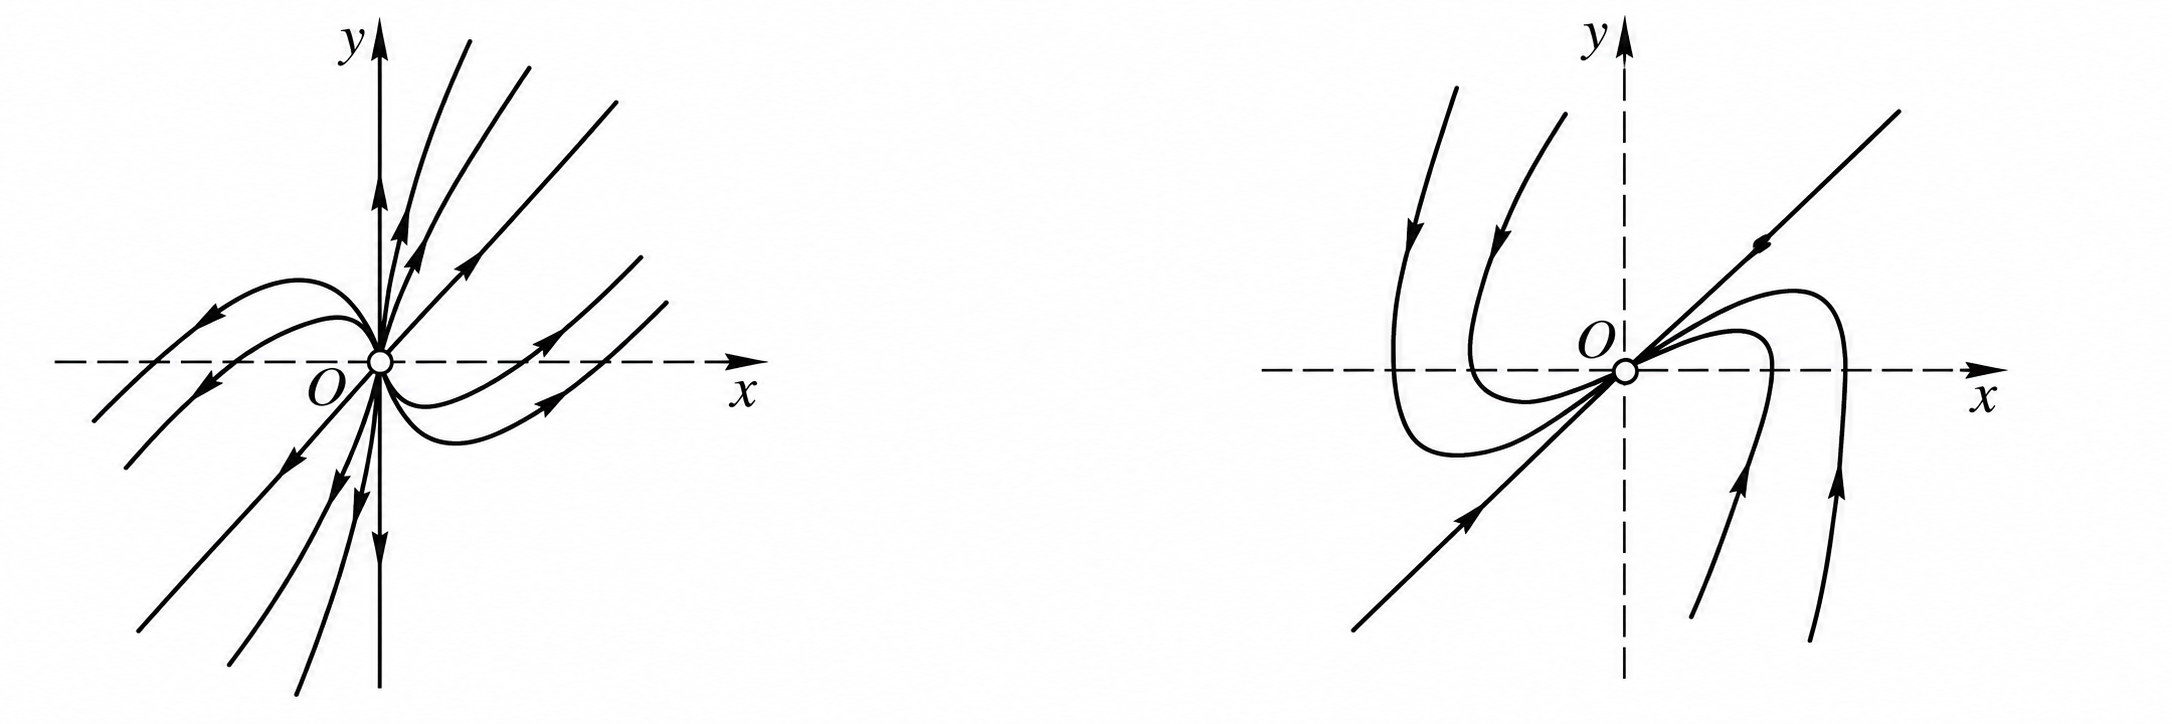
\includegraphics[width=0.7\linewidth]{figure/222}
	\label{fig:平面线性系统两例相图}
	\captionof{figure}{平面线性系统两例相图}
\end{center}


以上讨论了系数矩阵 $A$ 没有零特征根的各种情形。所有上述类型的
平衡点都称为\textbf{初等平衡点}，否则称为\textbf{退化平衡点}
（或\textbf{高阶平衡点}）。除中心以外的初等平衡点称为\textbf{粗的}，
其余平衡点称为\textbf{细的}。

下面一些内容的详细证明将在进一步关于常微分方程的学习中涉猎。
\begin{theorem}
	若非线性系统的线性部分具有粗的平衡点 $O$，则非线性系统在原点的
小邻域内与线性化系统具有相同的定性性质。
\end{theorem}
事实上，这时线性化系统的
特征根实部都不为零；即使原系统作微小改变，平衡点附近轨道的拓扑结构
仍与线性化系统相同。对于细的平衡点，非线性系统与其线性化系统未必
具有这种一致性。例如，线性部分为中心时，非线性系统的平衡点也可能
是焦点，这类情形需要进一步作中心焦点判定。

最后考虑退化平衡点，即 $\det A=0$。线性系统的特征方程为
\[
	\lambda^2-(a+d)\lambda=0,
\]
故特征根为
\[
	\lambda_1=0,
	\qquad
	\lambda_2=a+d.
\]
当 $a\neq0$ 或 $b\neq0$ 时，系统可写成
\[
	\dfrac{\dd x}{\dd t}=ax+by,
	\qquad
	\dfrac{\dd y}{\dd t}=k(ax+by),
\]
其中 $k$ 为常数。直线 $ax+by=0$ 上的所有点都是平衡点，称为
\textbf{奇线}。相空间中的轨道满足
\[
	\dfrac{\dd y}{\dd x}=k,
\]
因而是一族平行直线
\[
	y=kx+C_0.
\]
另一方面，沿轨道有
\[
	\dfrac{\dd}{\dd t}(ax+by)=\lambda_2(ax+by),
\]
从而
\[
	ax+by=C_1e^{\lambda_2t}.
\]
因此，当 $\lambda_2<0$ 时轨道趋近奇线上的点；当 $\lambda_2>0$ 时
轨道远离奇线上的点，相图见图 \ref{fig:非孤立退化平衡点相图}。
\newpage
\begin{center}
	\begin{tikzpicture}[>=Stealth,x=1cm,y=1cm]
		% a+d<0：轨道从两侧趋向奇线
		\begin{scope}[shift={(-3.45,0)}]
			\begin{scope}
				\clip (-2.5,-1.75) rectangle (2.5,2.05);
				\foreach \c in {-1.4,-.7,0,.7,1.4}{
					\pgfmathsetmacro{\ix}{\c/1.47}
					\pgfmathsetmacro{\iy}{.75*\ix}
					\draw[gray!75]
						plot[domain=-2.7:2.7,samples=2]
						(\x,{-.72*\x+\c});
					\draw[->]
						({\ix-1.05},{\iy+.756}) --
						({\ix-.13},{\iy+.0936});
					\draw[->]
						({\ix+1.05},{\iy-.756}) --
						({\ix+.13},{\iy-.0936});
					\fill[white] (\ix,\iy) circle (2.2pt);
					\draw (\ix,\iy) circle (2.2pt);
				}
				\draw[thick] (-2.35,-1.7625) -- (2.35,1.7625);
			\end{scope}
			\draw[->] (-2.55,0)--(2.55,0) node[right] {$x$};
			\draw[->] (0,-1.8)--(0,2.1) node[above] {$y$};
			\node[fill=white,inner sep=1pt,anchor=west]
				at (.72,.72) {$ax+by=0$};
			\node[below left] at (0,0) {$O$};
			\node at (0,-2.18) {$a^2+b^2\neq0$ 且 $a+d<0$};
		\end{scope}

		% a+d>0：轨道从奇线向两侧离开
		\begin{scope}[shift={(3.45,0)}]
			\begin{scope}
				\clip (-2.5,-1.75) rectangle (2.5,2.05);
				\foreach \c in {-1.4,-.7,0,.7,1.4}{
					\pgfmathsetmacro{\ix}{\c/1.47}
					\pgfmathsetmacro{\iy}{.75*\ix}
					\draw[gray!75]
						plot[domain=-2.7:2.7,samples=2]
						(\x,{-.72*\x+\c});
					\draw[->]
						({\ix-.13},{\iy+.0936}) --
						({\ix-1.05},{\iy+.756});
					\draw[->]
						({\ix+.13},{\iy-.0936}) --
						({\ix+1.05},{\iy-.756});
					\fill[white] (\ix,\iy) circle (2.2pt);
					\draw (\ix,\iy) circle (2.2pt);
				}
				\draw[thick] (-2.35,-1.7625) -- (2.35,1.7625);
			\end{scope}
			\draw[->] (-2.55,0)--(2.55,0) node[right] {$x$};
			\draw[->] (0,-1.8)--(0,2.1) node[above] {$y$};
			\node[fill=white,inner sep=1pt,anchor=west]
				at (.72,.72) {$ax+by=0$};
			\node[below left] at (0,0) {$O$};
			\node at (0,-2.18) {$a^2+b^2\neq0$ 且 $a+d>0$};
		\end{scope}
	\end{tikzpicture}
	\captionof{figure}{奇线附近轨道的趋近与远离}
	\label{fig:非孤立退化平衡点相图}
\end{center}

若 $\lambda_2=0$，则 $A$ 的两个特征根都为零，并且
$a+kb=0$。系统的通解为
\[
	x(t)=bC_0t+C_2,
	\qquad
	y(t)=dC_0t+(kC_2+C_0),
\]
其中 $C_0,C_2$ 为任意常数。此时轨道仍与奇线平行，轨道的走向由
$b,d,C_0$ 的符号确定，奇线将相平面分成的两部分中，轨道走向相反。
图 \ref{fig:双零特征根退化平衡点相图} 给出了 $b<0$、$d<0$
且 $a+d=0$ 时的相图。

\begin{center}
	\begin{tikzpicture}[>=Stealth,x=1cm,y=1cm]
		\begin{scope}
			\clip (-2.55,-2.05) rectangle (2.55,2.25);

			% 与奇线平行的轨道族
			\foreach \c in {-1.4,-.7,0,.7,1.4}{
				\draw[gray!75]
					plot[domain=-2.8:2.8,samples=2]
					(\x,{.78*\x+\c});
			}

			% 奇线上方的轨道向左下方运动
			\foreach \c in {.7,1.4}{
				\draw[->]
					(1.15,{.78*1.15+\c}) --
					(.20,{.78*.20+\c});
			}

			% 奇线下方的轨道向右上方运动
			\foreach \c in {-.7,-1.4}{
				\draw[->]
					(-1.15,{.78*(-1.15)+\c}) --
					(-.20,{.78*(-.20)+\c});
			}

			% 奇线由平衡点组成
			\draw[thick] (-2.45,-1.911) -- (2.45,1.911);
			\foreach \x in {-.72,0,.72}{
				\fill[white] (\x,{.78*\x}) circle (2.2pt);
				\draw (\x,{.78*\x}) circle (2.2pt);
			}
		\end{scope}

		\draw[dashed,->] (-2.65,0)--(2.65,0) node[right] {$x$};
		\draw[dashed,->] (0,-2.1)--(0,2.3) node[above] {$y$};
		\node[fill=white,inner sep=1pt,rotate=38]
			at (.95,.94) {$ax+by=0$};
		\node[below right] at (0,0) {$O$};
		\node at (0,-2.45) {$b<0,\ d<0$ 且 $a+d=0$};
	\end{tikzpicture}
	\captionof{figure}{双零特征根情形下奇线附近的轨道}
	\label{fig:双零特征根退化平衡点相图}
\end{center}

若 $a=b=0$，但 $c,d$ 不全为零，则 $cx+dy=0$ 为奇线，轨道是一族
平行于 $y$ 轴的直线。当 $d<0$ 时轨道趋近奇线，当 $d>0$ 时轨道
远离奇线，相图见图 \ref{fig:a等于b等于零退化平衡点相图}。
若 $a=b=c=d=0$，则平衡点充满整个相平面。

\begin{center}
	\begin{tikzpicture}[>=Stealth,x=1cm,y=1cm]
		% d<0：竖直轨道趋向奇线
		\begin{scope}[shift={(-3.35,0)}]
			\begin{scope}
				\clip (-2.35,-2.05) rectangle (2.35,2.2);
				\foreach \x in {-1.5,-.75,0,.75,1.5}{
					\pgfmathsetmacro{\iy}{.72*\x}
					\draw[gray!75] (\x,-2.2)--(\x,2.3);
					\draw[->] (\x,{\iy+1.18})--(\x,{\iy+.14});
					\draw[->] (\x,{\iy-1.18})--(\x,{\iy-.14});
					\fill[white] (\x,\iy) circle (2.2pt);
					\draw (\x,\iy) circle (2.2pt);
				}
				\draw[thick] (-2.35,-1.692)--(2.35,1.692);
			\end{scope}
			\draw[dashed,->] (-2.45,0)--(2.45,0) node[right] {$x$};
			\draw[dashed,->] (0,-2.1)--(0,2.3) node[above] {$y$};
			\node[fill=white,inner sep=1pt,anchor=west]
				at (.72,.72) {$cx+dy=0$};
			\node[below right] at (0,0) {$O$};
			\node at (0,-2.4) {$a=b=0$ 且 $d<0$};
		\end{scope}

		% d>0：竖直轨道远离奇线
		\begin{scope}[shift={(3.35,0)}]
			\begin{scope}
				\clip (-2.35,-2.05) rectangle (2.35,2.2);
				\foreach \x in {-1.5,-.75,0,.75,1.5}{
					\pgfmathsetmacro{\iy}{.72*\x}
					\draw[gray!75] (\x,-2.2)--(\x,2.3);
					\draw[->] (\x,{\iy+.14})--(\x,{\iy+1.18});
					\draw[->] (\x,{\iy-.14})--(\x,{\iy-1.18});
					\fill[white] (\x,\iy) circle (2.2pt);
					\draw (\x,\iy) circle (2.2pt);
				}
				\draw[thick] (-2.35,-1.692)--(2.35,1.692);
			\end{scope}
			\draw[dashed,->] (-2.45,0)--(2.45,0) node[right] {$x$};
			\draw[dashed,->] (0,-2.1)--(0,2.3) node[above] {$y$};
			\node[fill=white,inner sep=1pt,anchor=west]
				at (.72,.72) {$cx+dy=0$};
			\node[below right] at (0,0) {$O$};
			\node at (0,-2.4) {$a=b=0$ 且 $d>0$};
		\end{scope}
	\end{tikzpicture}
	\captionof{figure}{$a=b=0$ 时奇线附近的轨道}
	\label{fig:a等于b等于零退化平衡点相图}
\end{center}

\section{周期轨道与 Poincar\'e 映射}\label{sec:周期轨道与Poincare映射}

一个孤立的闭轨称为\textbf{极限环}。这里所谓孤立，是指在它的充分小邻域内不存在其他闭轨。极限环必为其他轨道的极限集合。

设 $\Gamma$ 是一个极限环，则在 $\Gamma$ 的内、外两侧均可取充分小的邻域，使其中不再含有其他闭轨。这些邻域内的轨道或者趋于 $\Gamma$，或者离开 $\Gamma$。由此可将极限环分为以下三类。

\begin{definition}[极限环的稳定性]
	\label{def:极限环的稳定性}
	设 $\Gamma$ 是极限环。
	\begin{enumerate}
		\item 当 $t\to+\infty$ 时，$\Gamma$ 内、外两侧的轨道都螺旋地趋于 $\Gamma$，则称 $\Gamma$ 为\textbf{稳定极限环}；
		\item 当 $t\to-\infty$ 时，$\Gamma$ 内、外两侧的轨道都螺旋地趋于 $\Gamma$，则称 $\Gamma$ 为\textbf{不稳定极限环}；
		\item 若 $\Gamma$ 一侧的轨道在 $t\to+\infty$ 时趋于 $\Gamma$，而另一侧的轨道在 $t\to-\infty$ 时趋于 $\Gamma$，则称 $\Gamma$ 为\textbf{半稳定极限环}。
	\end{enumerate}
\end{definition}

\begin{center}
	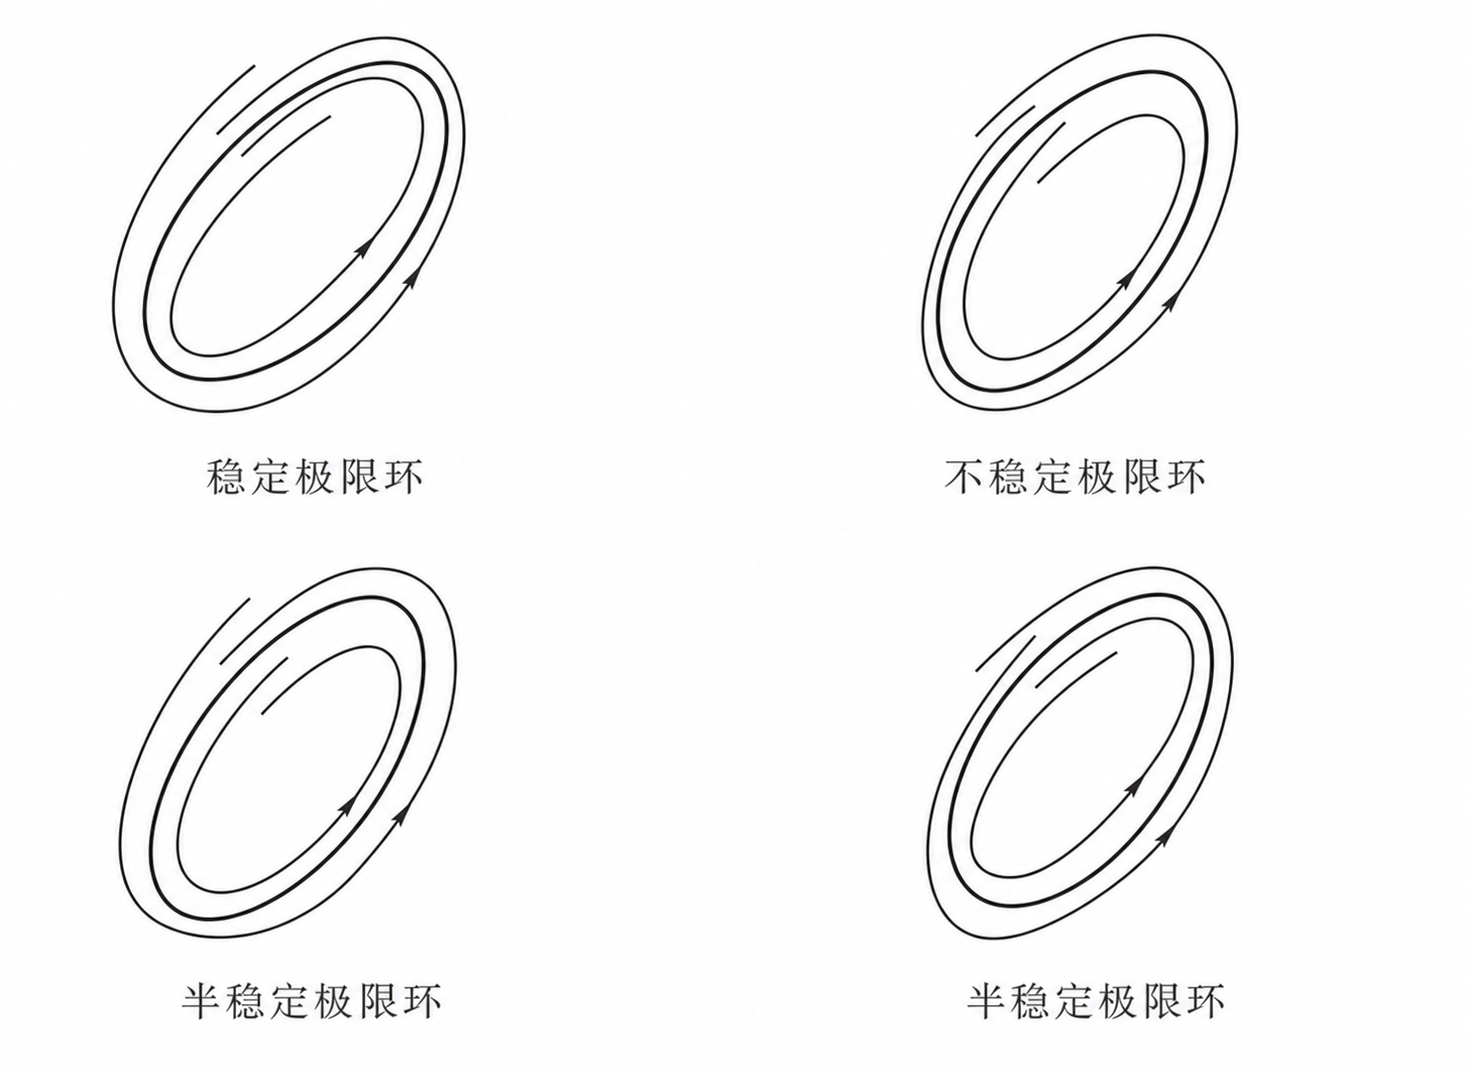
\includegraphics[width=0.6\linewidth]{figure/4}
\end{center}

平衡点和闭轨都可以成为轨道的极限状态。为了更准确地描述这一现象，给出如下定义。

\begin{definition}[$\omega$ 极限集合与 $\alpha$ 极限集合]
	\label{def:极限集合}
	设自治系统过 $\vect x_0$ 的轨道为 $\vect x=\vect \varphi(t,\vect x_0)$。若存在序列 $t_n\to+\infty$，使
	\[
		\vect \varphi(t_n,x_0)\to \vect x^*,
	\]
	则称 $\vect x^*$ 为轨道的一个 $\omega$ 极限点；所有 $\omega$ 极限点组成的集合称为 $\omega$ 极限集合，记为 $\omega(\vect x_0,\vect \varphi)$。类似地，以 $t_n\to-\infty$ 定义 $\alpha$ 极限点和 $\alpha$ 极限集合 $\alpha(\vect x_0,\vect \varphi)$。轨道的极限集合定义为
	\[
		L(\vect x_0,\vect \varphi):=\omega(\vect x_0,\vect \varphi)\cup\alpha(\vect x_0,\vect \varphi).
	\]
\end{definition}

若一条轨道是平衡点或闭轨，则它的 $\omega$ 极限集合和 $\alpha$ 极限集合都是轨道本身。由于 Jordan 曲线定理\footnote{也就是平面上任一简单闭曲线$\gamma$把平面分割为两部分，连接这两部分中任意点的连续路径必与$\gamma$相交。}，平面自治系统的极限集合具有较为简单的结构。

\begin{theorem}(Poincar\'e--Bendixson 环域定理)
	\label{thm:PoincareBendixson环域定理}
	设 $X(x,y),Y(x,y)$ 在区域 $G$ 内连续可微，$\overline D$ 是 $G$ 内的有界环形闭区域，并且
	\[
		\overline D=L_1\cup D\cup L_2,
	\]
	其中 $L_1$、$L_2$ 分别是 $\overline D$ 的内、外边界，均为简单闭曲线且都不是闭轨。若 $\overline D$ 内没有平衡点，并且从 $L_1$、$L_2$ 出发的轨道或者都不能离开 $\overline D$，或者都不能进入 $\overline D$，则 $D$ 内至少存在一条闭轨 $\Gamma$。
\end{theorem}

\begin{center}
	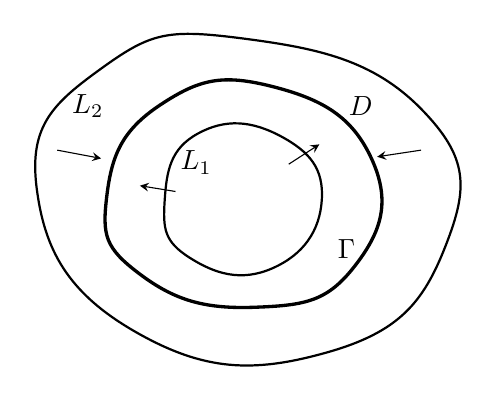
\begin{tikzpicture}[>=stealth,scale=1.05]
		\draw[thick] plot[smooth cycle,tension=.85] coordinates {(-2.4,.2) (-1.6,1.65) (.1,2) (2.25,1.15) (2.55,-.5) (1.1,-1.8) (-1.2,-1.55)};
		\draw[thick] plot[smooth cycle,tension=.85] coordinates {(-.85,.05) (-.45,.85) (.55,.82) (1.05,.05) (.45,-.78) (-.55,-.65)};
		\draw[very thick] plot[smooth cycle,tension=.85] coordinates {(-1.55,.1) (-.9,1.2) (.45,1.42) (1.65,.55) (1.45,-.75) (.25,-1.25) (-1.15,-.85)};
		\node at (-1.78,1.18) {$L_2$};
		\node at (-.47,.50) {$L_1$};
		\node at (1.52,1.18) {$D$};
		\node at (1.35,-.55) {$\Gamma$};
		\draw[->] (-2.15,.65)--(-1.62,.55);
		\draw[->] (2.25,.65)--(1.72,.57);
		\draw[->] (-.72,.15)--(-1.15,.22);
		\draw[->] (.65,.48)--(1.02,.72);
	\end{tikzpicture}
	\captionof{figure}{Poincar\'e--Bendixson 环域定理中的环形区域}
	\label{fig:PoincareBendixson环域}
\end{center}

在图~\ref{fig:PoincareBendixson环域} 中，$L_1$、$L_2$ 分别为环形区域的内、外边界。利用定理~\ref{thm:PoincareBendixson环域定理}，不仅可以证明闭轨的存在性，还可以通过选取较窄的环形区域来估计闭轨所在的位置。

\paragraph{例 6.6}
考虑系统
\[
	\begin{cases}
		x'=y+x(1-x^2-y^2),\\
		y'=-x+y(1-x^2-y^2).
	\end{cases}
\]
该系统只有一个平衡点 $O$。取
\[
	L_1:x^2+y^2=r_1^2<1,\qquad
	L_2:x^2+y^2=r_2^2>1,
\]
并以 $L_1,L_2$ 为内、外边界构成环形区域 $D$。令
\[
	V(x,y)=x^2+y^2,
\]
则沿系统的轨道有
\[
	\begin{aligned}
		\dfrac{\mathrm dV}{\mathrm dt}
		&=2x\bigl[y+x(1-x^2-y^2)\bigr]
		 +2y\bigl[-x+y(1-x^2-y^2)\bigr]\\
		&=2(x^2+y^2)(1-x^2-y^2).
	\end{aligned}
\]
因此，在 $L_1$ 上 $\dfrac{\mathrm dV}{\mathrm dt}>0$，在 $L_2$ 上 $\dfrac{\mathrm dV}{\mathrm dt}<0$，两条边界上的轨道都进入 $D$。由 Poincar\'e--Bendixson 环域定理，$D$ 内存在闭轨。

作极坐标变换
\[
	x=r\cos\theta,\qquad y=r\sin\theta,
\]
可得
\[
	\dfrac{\mathrm dr}{\mathrm dt}=r(1-r^2),\qquad
	\dfrac{\mathrm d\theta}{\mathrm dt}=-1.
\]
其解为
\[
	r(t)=\dfrac{1}{\sqrt{1+Ce^{-2t}}},\qquad
	\theta(t)=-(t-t_0),
\]
即
\[
	x(t)=\dfrac{\cos(t-t_0)}{\sqrt{1+Ce^{-2t}}},\qquad
	y(t)=\dfrac{-\sin(t-t_0)}{\sqrt{1+Ce^{-2t}}}.
\]
当 $C=0$ 时，得到闭轨
\[
	\Gamma:x^2+y^2=1.
\]
当 $C>0$ 时，轨道从 $\Gamma$ 内侧螺旋地趋于 $\Gamma$；当 $C<0$ 时，轨道从 $\Gamma$ 外侧螺旋地趋于 $\Gamma$。因此，$\Gamma$ 是系统唯一的稳定极限环，其相图如图~\ref{fig:示例稳定极限环相图} 所示。

\begin{center}
	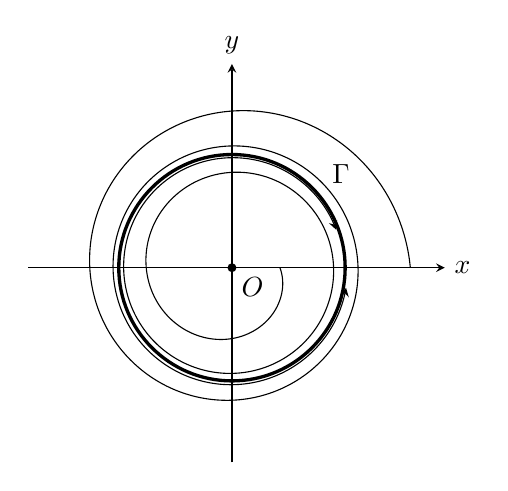
\begin{tikzpicture}[>=stealth,scale=1.15]
		\draw[->] (-2.25,0)--(2.35,0) node[right] {$x$};
		\draw[->] (0,-2.15)--(0,2.25) node[above] {$y$};
		\draw[very thick] (0,0) circle (1.25);
		\draw[->,domain=0:710,samples=260,smooth,variable=\t]
			plot ({(1.25+.72*exp(-.0045*\t))*cos(\t)},
			      {(1.25+.72*exp(-.0045*\t))*sin(\t)});
		\draw[->,domain=0:700,samples=260,smooth,variable=\t]
			plot ({(1.25-.72*exp(-.0048*\t))*cos(-\t)},
			      {(1.25-.72*exp(-.0048*\t))*sin(-\t)});
		\fill (0,0) circle (1.4pt) node[below right] {$O$};
		\node[above right] at (1.0,.82) {$\Gamma$};
	\end{tikzpicture}
	\captionof{figure}{例 6.6 的相图}
	\label{fig:示例稳定极限环相图}
\end{center}

下面给出两个判定平面自治系统不存在闭轨的准则。

\begin{theorem}[Bendixson 判据]
	\label{thm:Bendixson判据}
	设 $X(x,y),Y(x,y)$ 在区域 $G$ 内连续可微。若在单连通区域 $D\subset G$ 内，函数
	\[
		\dfrac{\partial X}{\partial x}+\dfrac{\partial Y}{\partial y}
	\]
	不变号，并且在 $D$ 的任何子区域内不恒等于零，则系统在 $D$ 内不存在闭轨。
\end{theorem}

\begin{proof}
	反设 $D$ 内存在闭轨 $\Gamma$，其参数方程为
	\[
		x=x(t),\qquad y=y(t),\qquad 0\leqslant t\leqslant T,
	\]
	并以 $D_0$ 表示 $\Gamma$ 所围成的区域。由 Green 公式，
	\[
		\begin{aligned}
			\iint_{D_0}\left(
			\dfrac{\partial X}{\partial x}
			+\dfrac{\partial Y}{\partial y}\right)\mathrm dx\mathrm dy
			&=\oint_{\Gamma}X\,\mathrm dy-Y\,\mathrm dx\\
			&=\int_0^T\left(X\dfrac{\mathrm dy}{\mathrm dt}
			-Y\dfrac{\mathrm dx}{\mathrm dt}\right)\mathrm dt=0.
		\end{aligned}
	\]
	但由假设，上述二重积分不可能为零，矛盾。
\end{proof}

\begin{theorem}[Dulac 判据]
	\label{thm:Dulac判据}
	设 $X(x,y),Y(x,y)$ 在区域 $G$ 内连续可微。若在单连通区域 $D\subset G$ 内存在连续可微函数 $B(x,y)$，使
	\[
		\dfrac{\partial(BX)}{\partial x}
		+\dfrac{\partial(BY)}{\partial y}
	\]
	不变号，并且在 $D$ 的任何子区域内不恒等于零，则系统在 $D$ 内不存在闭轨。函数 $B(x,y)$ 称为\textbf{Dulac 函数}。
\end{theorem}

寻找 Dulac 函数同寻找 Lyapunov 函数一样，需要一定的技巧。

\begin{proof}
	若 $D$ 内存在闭轨 $\Gamma$，设其围成区域为 $D_0$。由 Green 公式及 $\dot x=X,\dot y=Y$，有
	\[
		\begin{aligned}
			\iint_{D_0}\left[
			\dfrac{\partial(BX)}{\partial x}
			+\dfrac{\partial(BY)}{\partial y}\right]\mathrm dx\mathrm dy
			&=\oint_{\Gamma}BX\,\mathrm dy-BY\,\mathrm dx\\
			&=\int_0^T B(x(t),y(t))
			\left(X\dfrac{\mathrm dy}{\mathrm dt}
			-Y\dfrac{\mathrm dx}{\mathrm dt}\right)\mathrm dt=0.
		\end{aligned}
	\]
	这与被积函数不变号且在任何子区域内不恒为零矛盾。
\end{proof}

下面介绍后继函数。设原点 $O$ 是系统的中心型平衡点，即其线性化系统的平衡点为中心。为判别非线性系统的原点究竟是中心还是焦点，并研究原点附近闭轨的个数，需要考察相邻轨道在一条横截线上的交点。

在 $O$ 的充分小邻域 $B_\delta$ 内，非线性系统等价于本章前面给出的标准形式，其中非线性项充分小。取正 $x$ 轴为 $\Sigma$，令 $\Sigma_0=\Sigma\cap B_\delta$，并任取 $P_0\in\Sigma_0$。线性系统从 $P_0$ 出发的轨道经过一周后回到 $P_0$。由解对初值的连续依赖性，非线性系统从 $P_0$ 出发的轨道经过一周后与 $\Sigma_0$ 交于 $P_1$，且 $P_1$ 接近 $P_0$。于是可以定义映射
\[
	\Pi:\Sigma_0\longrightarrow\Sigma,\qquad
	\Pi(P_0)=P_1.
\]

\begin{definition}[Poincar\'e 映射]
	\label{def:Poincare映射}
	上述 $\Sigma_0$ 称为系统的一个\textbf{Poincar\'e 截面}，或称\textbf{横截线}；映射 $\Pi$ 称为\textbf{Poincar\'e 映射}。函数
	\[
		d(P):=\Pi(P)-P
	\]
	称为\textbf{后继函数}。
\end{definition}

原点附近的闭轨与 $\Pi$ 的不动点一一对应，即
\[
	\Pi(Q)=Q,\qquad Q\in\Sigma_0.
\]
若 $Q$ 是 $\Pi$ 的吸引不动点或排斥不动点，则后继函数在 $Q$ 两侧具有相应的符号变化，而与 $Q$ 对应的闭轨分别为稳定极限环或不稳定极限环。

\begin{center}
	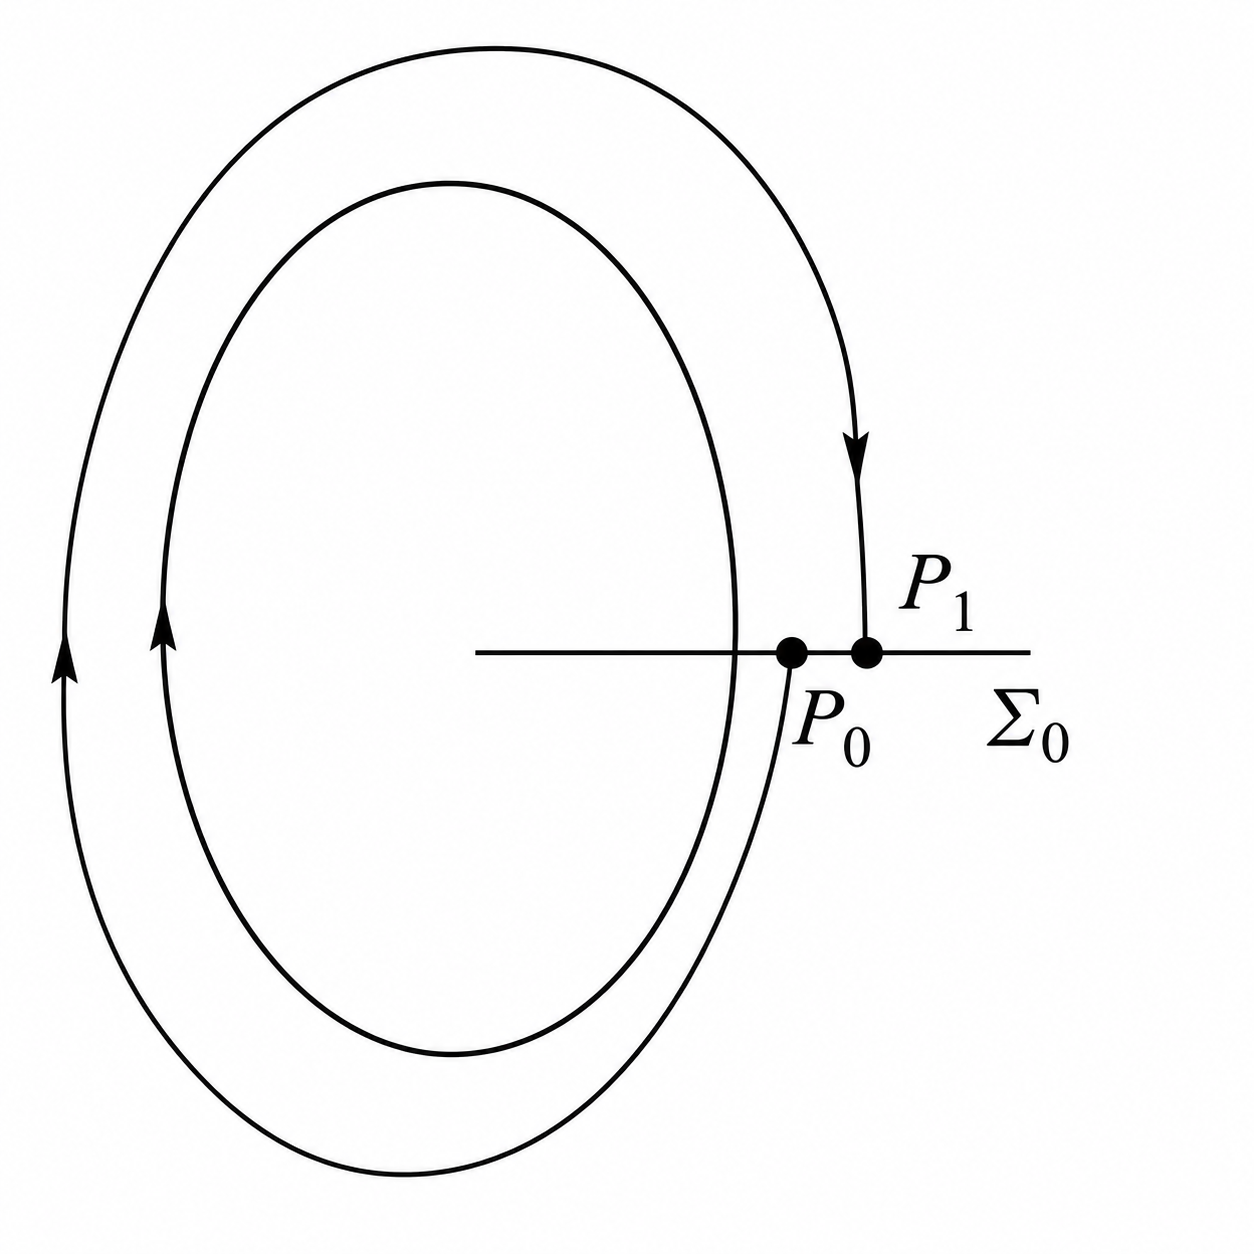
\includegraphics[width=0.5\linewidth]{figure/5}
	
	\captionof{figure}{Poincar\'e 映射与后继函数}
	\label{fig:Poincare映射}
\end{center}

Poincar\'e 映射把连续的轨道运动化为映射的迭代，因此将连续动力系统与离散动力系统联系起来。

\begin{definition}[离散动力系统]
	\label{def:离散动力系统}
	设 $X\subset\mathbb R^n$，$f:X\to X$ 是连续自映射。令
	\[
		f^0(x)=x,\qquad
		f^k(x)=f\bigl(f^{k-1}(x)\bigr),\quad k=2,3,\ldots.
	\]
	则半群
	\[
		\{f^k:k=0,1,2,\ldots\}
	\]
	称为由 $f$ 生成的离散半动力系统。若 $f$ 是同胚，则还可以考虑群
	\[
		\{f^k:k=0,\pm1,\pm2,\ldots\}.
	\]
	这就是离散动力系统。
\end{definition}

连续过程可以通过取样离散化，离散过程也可以嵌入连续过程之中。对于同胚 $f:X\to X$，定义
\[
	\begin{aligned}
		\operatorname{Orb}_f(x_0)
		&=\{f^k(x_0):k=0,\pm1,\pm2,\ldots\},\\
		\operatorname{Orb}_f^+(x_0)
		&=\{f^k(x_0):k=0,1,2,\ldots\},\\
		\operatorname{Orb}_f^-(x_0)
		&=\{f^{-k}(x_0):k=0,1,2,\ldots\}.
	\end{aligned}
\]
它们分别称为 $x_0$ 的轨道、正半轨道和负半轨道。

若存在自然数 $p$，使 $f^p(x_0)=x_0$，则称 $x_0$ 为 $f$ 的\textbf{周期点}；使该等式成立的最小自然数 $p$ 称为 $x_0$ 的\textbf{周期}。也就是说，
\[
	f^p(x_0)=x_0,\qquad
	f^k(x_0)\ne x_0,\quad k=1,2,\ldots,p-1.
\]
周期为 $1$ 的点称为不动点。$f$ 的周期点集合与不动点集合分别记为 $\operatorname{Per}(f)$ 和 $\operatorname{Fix}(f)$。

对于一维区间上的连续映射 $f:I\to I$，若 $x_0$ 是周期为 $p$ 的周期点，且 $f^p$ 在 $x_0$ 处可微，则当
\[
	\left|(f^p)'(x_0)\right|<1
\]
时，$x_0$ 是稳定周期点；当
\[
	\left|(f^p)'(x_0)\right|>1
\]
时，$x_0$ 是不稳定周期点。类似的有稳定不动点与不稳定不动点。

\paragraph{例 6.8}
考虑 Logistic 映射
\[
	f_\lambda:I=[0,1]\longrightarrow I,\qquad
	f_\lambda(x)=\lambda x(1-x),\qquad \lambda\in[0,4].
\]
它有不动点
\[
	x_1=0,\qquad x_2=1-\dfrac{1}{\lambda}.
\]
当 $\lambda<1$ 时，只有不动点 $x_1$，并且它是稳定的；当 $1<\lambda<3$ 时，$x_1$ 变为不稳定不动点，同时产生稳定不动点 $x_2$；当 $\lambda>3$ 时，$x_2$ 变为不稳定不动点，并产生两个周期为 $2$ 的周期点
\[
	x_{\pm}=\dfrac{1}{2\lambda}
	\left(1+\lambda\pm\sqrt{(\lambda+1)(\lambda-3)}\right).
\]
它们由方程 $f_\lambda^2(x)=x$ 得到。当
\[
	3<\lambda<1+\sqrt6
\]
时，这两个周期点是稳定的。随着参数 $\lambda$ 继续增大，稳定周期轨道的周期依次由
\[
	1\longrightarrow2\longrightarrow4\longrightarrow8\longrightarrow\cdots
\]
不断加倍，这种现象称为\textbf{倍周期分岔}，也称为\textbf{Feigenbaum 分岔}。参数值
\[
	\lambda=1,\quad3,\quad1+\sqrt6,\quad\ldots
\]
称为分岔点。其分岔图见图~\ref{fig:Feigenbaum分岔现象}。

\begin{center}
	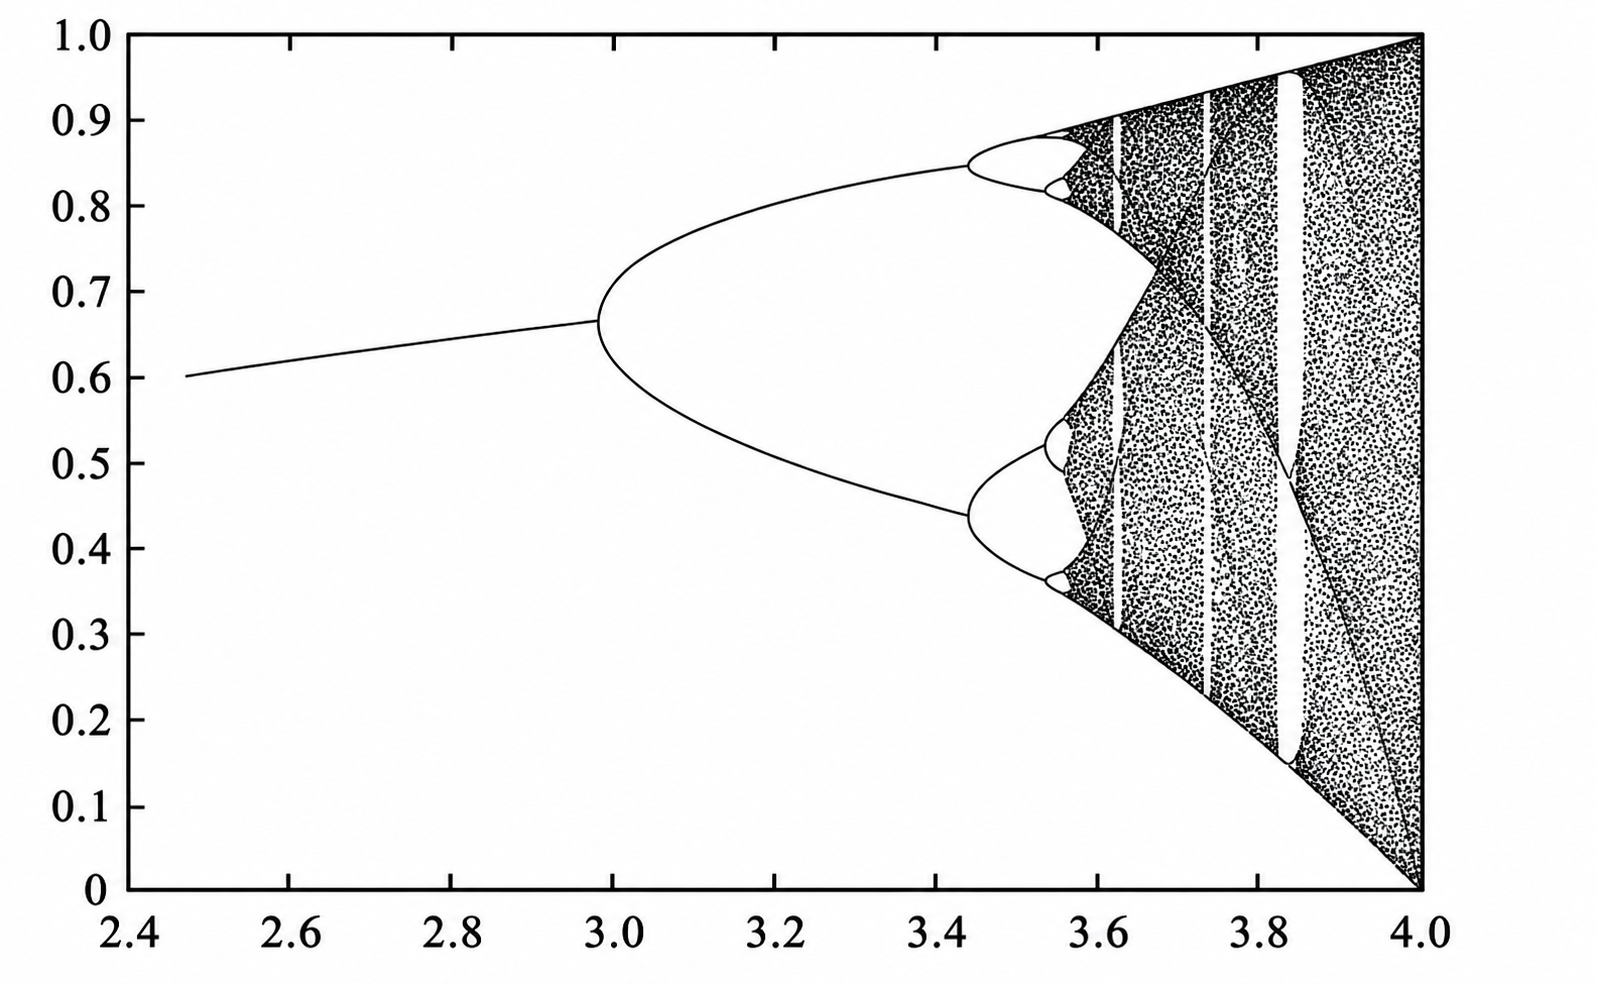
\includegraphics[width=0.7\linewidth]{figure/3}
	
	\captionof{figure}{Feigenbaum 分岔现象}
	\label{fig:Feigenbaum分岔现象}
\end{center}

1964年，Sharkovsky对自然数做了重新排序，对于闭区间上的连续自映射，其周期之间存在如下 Sharkovsky 次序：
\[
\begin{aligned}
	3&\triangleleft5\triangleleft7\triangleleft\cdots
	\triangleleft(2n+1)\triangleleft(2n+3)\triangleleft\cdots\\
	&\triangleleft2\cdot3\triangleleft2\cdot5\triangleleft2\cdot7\triangleleft\cdots\\
	&\triangleleft2^2\cdot3\triangleleft2^2\cdot5\triangleleft2^2\cdot7\triangleleft\cdots\\
	&\qquad\vdots\\
	&\triangleleft2^m\cdot3\triangleleft2^m\cdot5\triangleleft2^m\cdot7\triangleleft\cdots\\
	&\qquad\vdots\\
	&\triangleleft2^\ell\triangleleft2^{\ell-1}\triangleleft\cdots
	\triangleleft16\triangleleft8\triangleleft4\triangleleft2\triangleleft1.
\end{aligned}
\]
并证明了以下重要的结果，它全面揭示了一维迭代动力系统的周期性规律。
\begin{theorem}(Sharkovsky 定理)
	\label{thm:Sharkovsky定理}
	设 $I\subset\mathbb R$ 是闭区间，$f:I\to I$ 是连续自映射。若 $f$ 有周期为 $p$ 的周期点，则对每个自然数 $m$，只要
	\[
		p\triangleleft m,
	\]
	$f$ 就有周期为 $m$ 的周期点。
\end{theorem}

\section{平面 Hamilton 系统}\label{sec:平面Hamilton系统}

在这一节中，我们应用前面的定性理论方法来分析一类在物理学中重要的系统，即 Hamilton 系统。

\begin{definition}\label{def:Hamilton系统}
	令 $W\subset\mathbb R^{2n}$ 为开集，$\vect x,\vect y\in\mathbb R^n$，且 $(\vect x,\vect y)\in W$，$H(\vect x,\vect y)$ 为定义在 $W$ 上的连续可微实函数。称系统
	\[
		\dfrac{\dd \vect x}{\dd t}=\dfrac{\partial H}{\partial \vect y},
		\qquad
		\dfrac{\dd \vect y}{\dd t}=-\dfrac{\partial H}{\partial \vect x}
	\]
	为 $W$ 上带 $n$ 个自由度的 \textbf{Hamilton 系统}，称 $H(\vect x,\vect y)$ 为该系统的 \textbf{Hamilton 函数}。其中
	\[
	\begin{aligned}
		\vect x&=(x_1,x_2,\ldots,x_n)^{\mathrm T},
		&\vect y&=(y_1,y_2,\ldots,y_n)^{\mathrm T},\\
		\dfrac{\partial H}{\partial \vect x}
		&=\left(
		\dfrac{\partial H}{\partial x_1},
		\dfrac{\partial H}{\partial x_2},\ldots,
		\dfrac{\partial H}{\partial x_n}
		\right)^{\mathrm T},
		&
		\dfrac{\partial H}{\partial \vect y}
		&=\left(
		\dfrac{\partial H}{\partial y_1},
		\dfrac{\partial H}{\partial y_2},\ldots,
		\dfrac{\partial H}{\partial y_n}
		\right)^{\mathrm T}.
	\end{aligned}
	\]
\end{definition}

在经典天体力学的多体问题和无阻尼的机械振动中，常常会遇到 Hamilton 系统。这时 Hamilton 函数 $H(x,y)$ 往往表示相应力学系统的总能量，因此一般又称它为能量函数。下面给出 Hamilton 函数的一个重要性质。

\begin{theorem}(Hamilton 函数的守恒性)\label{thm:Hamilton函数沿轨道守恒}
	Hamilton 系统的 Hamilton 函数 $H(x,y)$ 沿该系统的轨道等于常数。
\end{theorem}

\begin{proof}
	设 $(x(t),y(t))$ 为 Hamilton 系统的解，则 $H(x(t),y(t))$ 是 $t$ 的函数，并且
	\[
	\begin{aligned}
		\dfrac{\dd}{\dd t}H(x(t),y(t))
		&=\dfrac{\partial H}{\partial x}\dfrac{\dd x}{\dd t}
		 +\dfrac{\partial H}{\partial y}\dfrac{\dd y}{\dd t}\\
		&=\dfrac{\partial H}{\partial x}\dfrac{\partial H}{\partial y}
		 -\dfrac{\partial H}{\partial y}\dfrac{\partial H}{\partial x}=0.
	\end{aligned}
	\]
	故沿着轨道 $(x(t),y(t))$，函数 $H(x,y)$ 为常数。
\end{proof}

上述定理表明，在无阻尼的机械振动系统中，系统的总能量保持不变，即 Hamilton 系统满足能量等值定律。一般把满足能量等值定律的系统称为保守系统，因此 Hamilton 系统是保守系统。

带一个自由度的 Hamilton 系统称为\textbf{平面 Hamilton 系统}。前面许多例子都涉及如下形式的微分方程：
\[
	\dfrac{\dd^2x}{\dd t^2}+g(x)=0,
\]
其中 $x\in\mathbb R$，$g(x)$ 为 $\mathbb R$ 上的连续可微函数。若用 $y$ 表示速度，则该方程等价于
\[
	\dfrac{\dd x}{\dd t}=y,
	\qquad
	\dfrac{\dd y}{\dd t}=-g(x).
\]
这是一个 Hamilton 系统，其 Hamilton 函数为
\[
	H(x,y)=\dfrac{y^2}{2}+G(x),
\]
其中
\[
	G(x)=\int_0^x g(s)\,\dd s.
\]
$G(x)$ 是系统运动的势能，$\dfrac{y^2}{2}$ 是系统运动的动能，因此这类特殊的平面 Hamilton 系统也称为“动能 $+$ 势能”型 Hamilton 系统。

容易看出，$(x_0,y_0)$ 为上述系统的平衡点，当且仅当
\[
	y_0=0,\qquad g(x_0)=0.
\]
在这种情形下 $G'(x_0)=0$，因此 $x_0$ 为势能函数 $G(x)$ 的临界点。

\begin{theorem}(平衡点的分类)\label{thm:动能加势能型Hamilton系统平衡点分类}
	上述系统的平衡点都在 $x$ 轴上，$(x_0,0)$ 为平衡点当且仅当 $x_0$ 为势能函数 $G(x)$ 的临界点。当 $x_0$ 为 $G(x)$ 的严格极大值点，即 $G''(x_0)<0$ 时，$(x_0,0)$ 为系统的鞍点；当 $x_0$ 为 $G(x)$ 的严格极小值点，即 $G''(x_0)>0$ 时，$(x_0,0)$ 为系统的中心。
\end{theorem}

\begin{proof}
	设 $x_0$ 为 $G(x)$ 的严格极大值点，则
	\[
		G'(x_0)=g(x_0)=0,
		\qquad
		G''(x_0)=g'(x_0)<0.
	\]
	在 $(x_0,0)$ 处，系统右端函数的 Jacobi 矩阵为
	\[
		A=\begin{pmatrix}
			0&1\\
			-g'(x_0)&0
		\end{pmatrix}.
	\]
	此时
	\[
		\operatorname{tr}A=0,
		\qquad
		\det A=g'(x_0)<0,
	\]
	故矩阵 $A$ 有两个符号相反的非零实特征根，因而 $(x_0,0)$ 为系统的鞍点。

	再设 $x_0$ 为 $G(x)$ 的严格极小值点，则
	\[
		G'(x_0)=g(x_0)=0,
		\qquad
		G''(x_0)=g'(x_0)>0.
	\]
	Jacobi 矩阵仍为上面的矩阵 $A$，同时
	\[
		\operatorname{tr}A=0,
		\qquad
		\det A=g'(x_0)>0.
	\]
	因此，矩阵 $A$ 的两个特征根是一对共轭纯虚根，故 $(x_0,0)$ 为系统线性部分的中心。

	为了进一步证明 $(x_0,0)$ 也是原系统的中心，由定理~\ref{thm:Hamilton函数沿轨道守恒}，系统在平衡点 $(x_0,0)$ 附近的轨道形成相平面中的一族曲线
	\[
		V(x,y)=\dfrac{y^2}{2}+G(x)-G(x_0)=C,
	\]
	其中 $C$ 为常数。显然 $V(x_0,0)=0$。又由于 $x_0$ 为 $G(x)$ 的严格极小值点，存在 $(x_0,0)$ 的闭邻域
	\[
		N_\delta=\left\{(x,y)\in\mathbb R^2:
		(x-x_0)^2+y^2\leqslant\delta^2\right\},
	\]
	使得在 $N_\delta\setminus\{(x_0,0)\}$ 上 $V(x,y)>0$。令
	\[
		l=\min_{(x,y)\in\partial N_\delta}V(x,y),
	\]
	其中
	\[
		\partial N_\delta=\left\{(x,y)\in\mathbb R^2:
		(x-x_0)^2+y^2=\delta^2\right\}
	\]
	是 $N_\delta$ 的边界。

	只要 $0<C<l$，曲线 $V(x,y)=C$ 就是包含平衡点 $(x_0,0)$ 在内的闭曲线。事实上，设 $\gamma$ 是由 $(x_0,0)$ 出发到 $\partial N_\delta$ 的任意一条曲线，则沿着 $\gamma$，$V(x,y)$ 的值由初始的 $0$ 变到大于或等于 $l$。对任意给定的常数 $0<C<l$，由 $V(x,y)$ 的连续性，$\gamma$ 上必有一点使 $V(x,y)=C$，即 $\gamma$ 必与曲线 $V(x,y)=C$ 相交。因此，该曲线必为包含平衡点 $(x_0,0)$ 在内的闭曲线。

	取定某个 $C_0<l$。当 $C$ 从 $0$ 变到 $C_0$ 时，由 $V(x,y)=C$ 得到一族彼此不相交并同时包含平衡点 $(x_0,0)$ 在内的闭曲线；当 $C=0$ 时，它退化为平衡点 $(x_0,0)$。因此，存在 $(x_0,0)$ 的一个邻域，使系统的轨道全为闭轨，从而 $(x_0,0)$ 为系统的中心。
\end{proof}
\begin{center}
	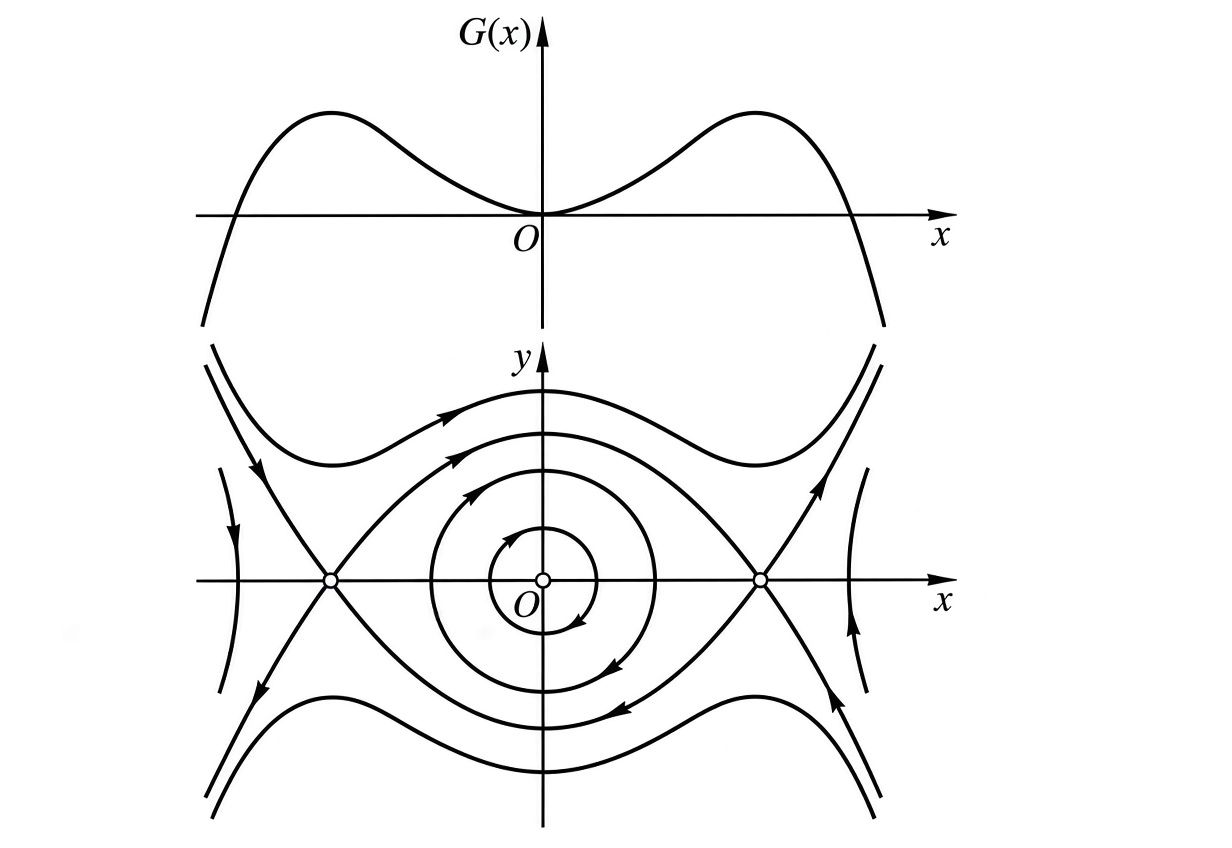
\includegraphics[width=0.7\linewidth]{figure/6}
	\captionof{figure}{系统的势能函数与相图}
\end{center}

由定理~\ref{thm:动能加势能型Hamilton系统平衡点分类}，如果势能函数 $G(x)$ 仅有孤立临界点，并且每个临界点都是严格极值点，就可以由 $G(x)$ 的图像在 $Oxy$ 坐标系中画出系统的相图，如图~\ref{fig:动能加势能型Hamilton系统相图} 所示。除平衡点均在 $x$ 轴上外，轨道由曲线族
\[
	H(x,y)=C
\]
给出，并且关于 $x$ 轴对称。


